% Chapter Template

\chapter{Results for High-Dimension Model Representation} % Main chapter title

\label{ch:results hdmr} % Change X to a consecutive number; for referencing this chapter elsewhere, use \ref{ChapterX}

\lhead{Chapter 6. \emph{Results: HDMR}} % Change X to a consecutive number; this is for the header on each page - perhaps a shortened title

%----------------------------------------------------------------------------------------
%	SECTION: INTRO
%----------------------------------------------------------------------------------------

\section{Introduction}
In this chapter we contrast results obtained using stochastic collocation for generalized polynomial chaos
expansions (SCgPC) and high-dimension model representation (HDMR) uncertainty quantification methods.  In each case
we also include Monte Carlo (MC) as a comparison benchmark.

As with SCgPC, the objective in introducing HDMR methods is to reduce the number of computational model solves
necessary to obtain reasonable second-order statistics for models.  The analytic models we use for initial
demonstration are described in Chapter \ref{ch:results scgpc}, along with the performance of SCgPC methods in
representing the same.  In this chapter, we add HDMR methods to the analysis, and consider their performance
in comparison to MC and SCgPC methods.

We consider three static HDMR cases as well as adaptive HDMR using adaptive SCgPC to expand subset terms.  In
static HDMR, each series represents an HDMR truncation level.  The HDMR truncation level determines the
maximum level of interactions allowable in the expansion.  For example, HDMR 1 includes only first-order
interactions.  We consider first-, second-, and third-order HDMR truncations.  For each of these truncations,
we use SCgPC expansions of growing polynomial order limit, with polynomials selected by using the total degree
index set construction method.  Each successive data point in each static series is obtained by increasing the
limiting total polynomial order $L$ for the subset terms.

As discussed in section \ref{sec:conv gpc hdmr}, we do not expect the convergence rate of the static HDMR
methods to exceed the convergence rate of their corresponding SCgPC counterparts.  However, there may be some
static HDMR constructions that require less computational solves than SCgPC methods.  In addition, we expect
the flexibility of the adaptive HDMR method to allow improved convergence over other methods for some models.

As in Chapter \ref{ch:results scgpc}, the performance of each method is analyzed using \emph{value figures}
and \emph{convergence figures} for both the mean and standard deviation of each model's response.  Value
figures will provide actual values obtained for the moments, while convergence figures show the relative error
of the values obtained to the analytic benchmark value.  Monte Carlo error bars are calculated as described in
Chapter \ref{ch:results scgpc}.

All computations shown here were performed using the \raven{} \cite{raven} framework.  As noted previously,
computations were written to file using 10 digits of accuracy.
As a result, any apparent convergence past this level of accuracy is coincidental or the result of
machine-exact values, and we consider a relative difference of $10^{-10}$ to be converged.

\section{Tensor Monomials}
This model is described in section \ref{mod:tensor monom}.  As the tensor product of linear polynomials, it is
very conducive to SCgPC.  Because all terms are equally important, however, truncating the HDMR expansion of
this model removes important elements, which makes HDMR less ideal for this model in general.

\subsection{3 Inputs}
With only three input parameters, we can clearly see the contribution of the first-order interaction terms,
second-order interaction terms, and third-order interaction terms from HDMR 1, HDMR 2, and HDMR 3.  As
expected, with only first-order polynomials HDMR 3 converges exactly; however, HDMR 1 and HDMR 2 neglect
critical polynomials in the expansion, and so are less suitable methods for this model.  Note also that after
first-order polynomials, adding additional polynomial orders does not reduce error for the static HDMR
methods, as no higher-order polynomials exist in the original model.
The adaptive HDMR method, however, performs admirably for this model, quickly finding the appropriate search
direction for the response dependencies and converging as rapidly as the adaptive SCgPC method.
\begin{figure}[H]
  \centering
  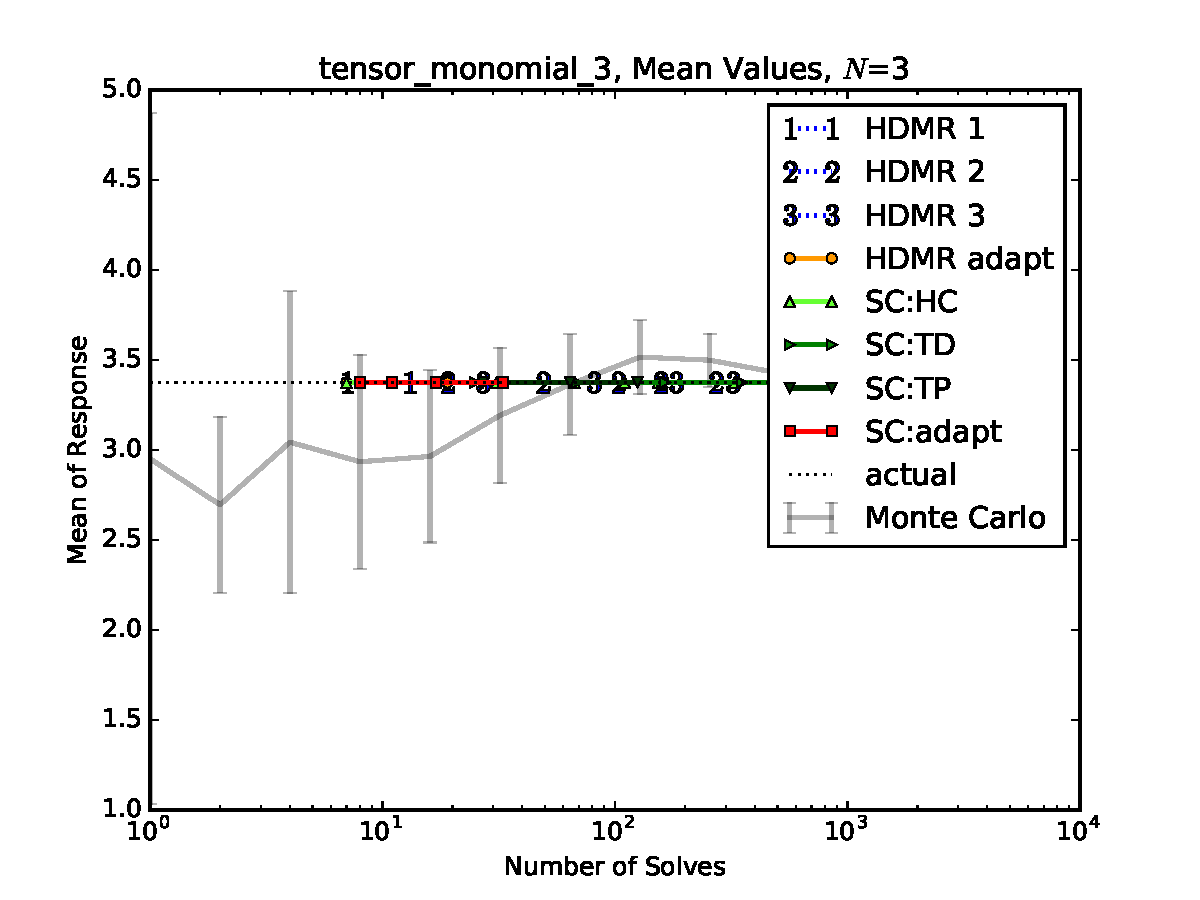
\includegraphics[width=0.7\linewidth]{anlmodels/tensor_monomial_3_mean_vals}
  \caption{Tensor Monomial, $N=3$, Mean Values}
  \label{fig:hdmr tensormono mean values 3}
\end{figure}
\begin{figure}[H]
  \centering
  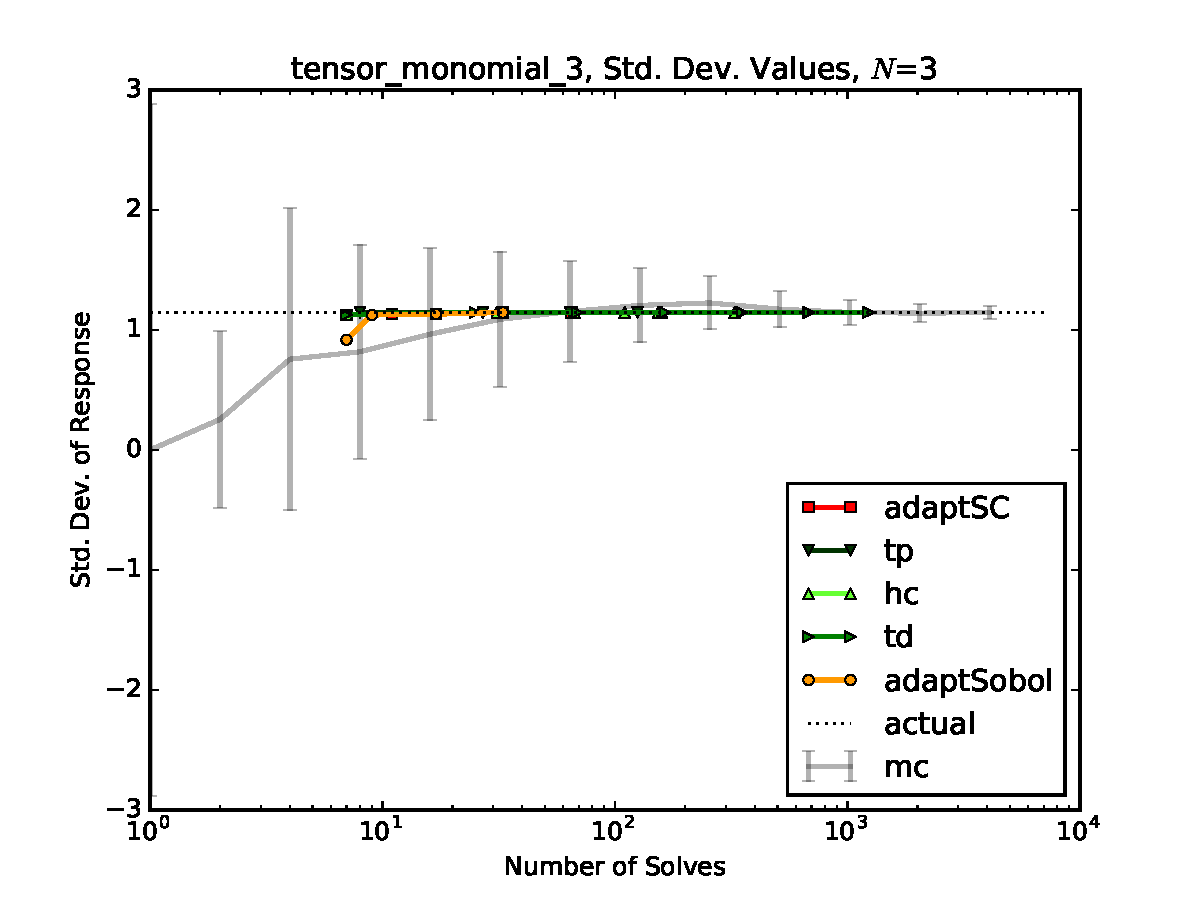
\includegraphics[width=0.7\linewidth]{anlmodels/tensor_monomial_3_var_vals}
  \caption{Tensor Monomial, $N=3$, Std. Dev. Values}
  \label{fig:hdmr tensormono var values 3}
\end{figure}

\begin{figure}[H]
  \centering
  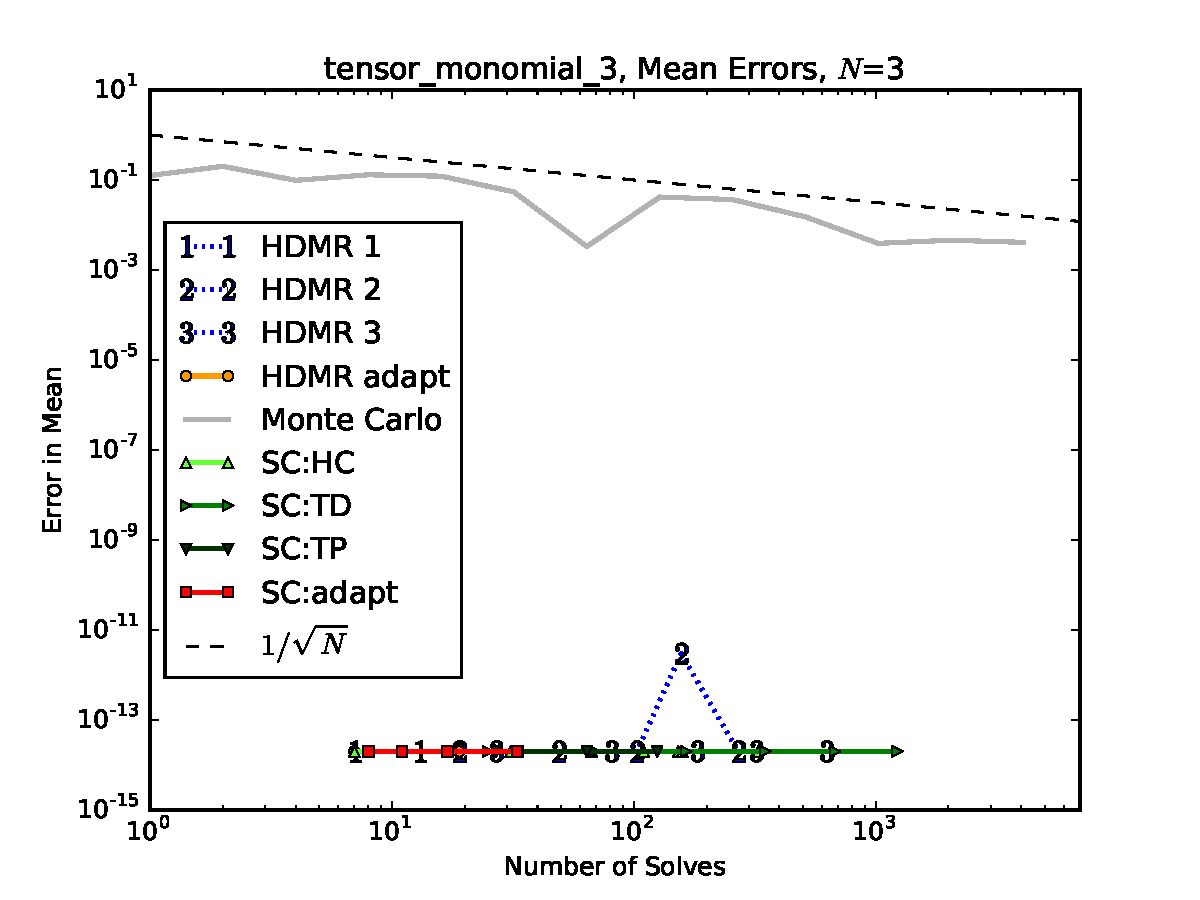
\includegraphics[width=0.7\linewidth]{anlmodels/tensor_monomial_3_mean_errs}
  \caption{Tensor Monomial, $N=3$, Mean Convergence}
  \label{fig:hdmr tensormono mean errors 3}
\end{figure}
\begin{figure}[H]
  \centering
  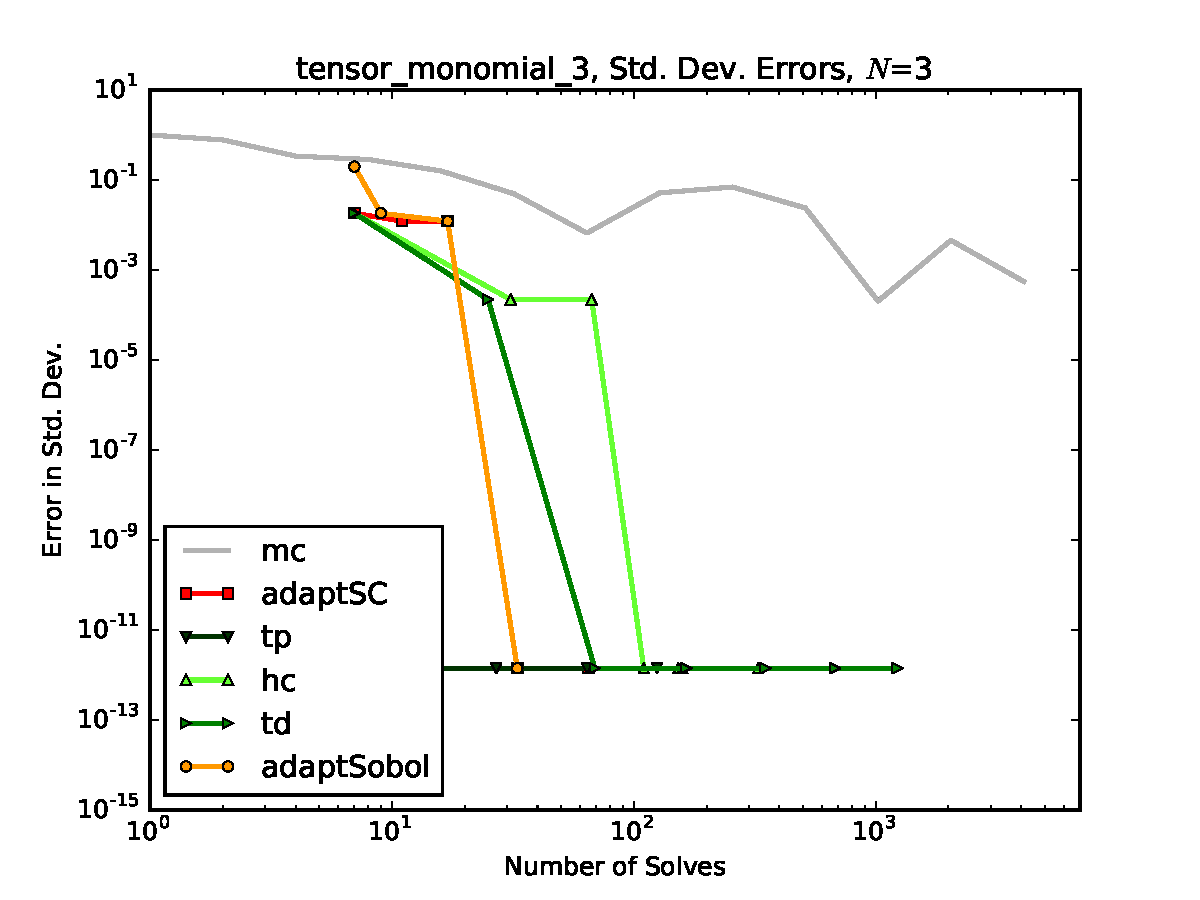
\includegraphics[width=0.7\linewidth]{anlmodels/tensor_monomial_3_variance_errs}
  \caption{Tensor Monomial, $N=3$, Std. Dev. Convergence}
  \label{fig:hdmr tensormono var errors 3}
\end{figure}




\subsection{5 Inputs}
Increasing the dimensionality serves to enforce those observations already recorded for the three-dimensional
input space.  HDMR methods perform no better than their SCgPC counterparts, and because of their truncation
are limited in their ability to converge the statistical moments for this model.  Interestingly, however, the
adaptive HDMR method outperforms the adaptive SCgPC method in finding the exact solution, because it searches
both subspaces to add as well as polynomials, and wastes less time searching higher-order polynomials that do
not exist in the expansion.  In essence, it eliminates portions of the Hilbert spaced spanned by the
bases polynomials more quickly than the adaptive SCgPC method.
\begin{figure}[H]
  \centering
  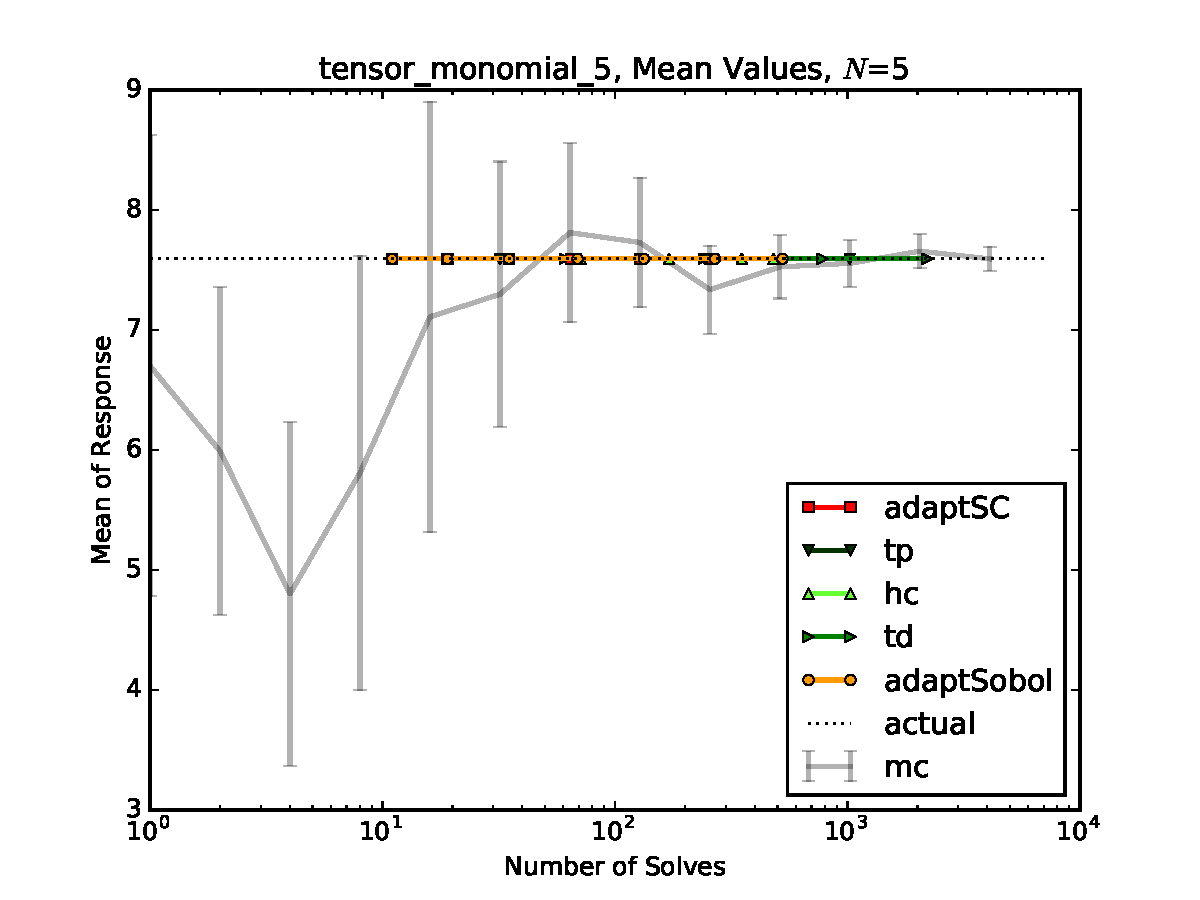
\includegraphics[width=0.7\linewidth]{anlmodels/tensor_monomial_5_mean_vals}
  \caption{Tensor Monomial, $N=5$, Mean Values}
  \label{fig:hdmr tensormono mean values 5}
\end{figure}
\begin{figure}[H]
  \centering
  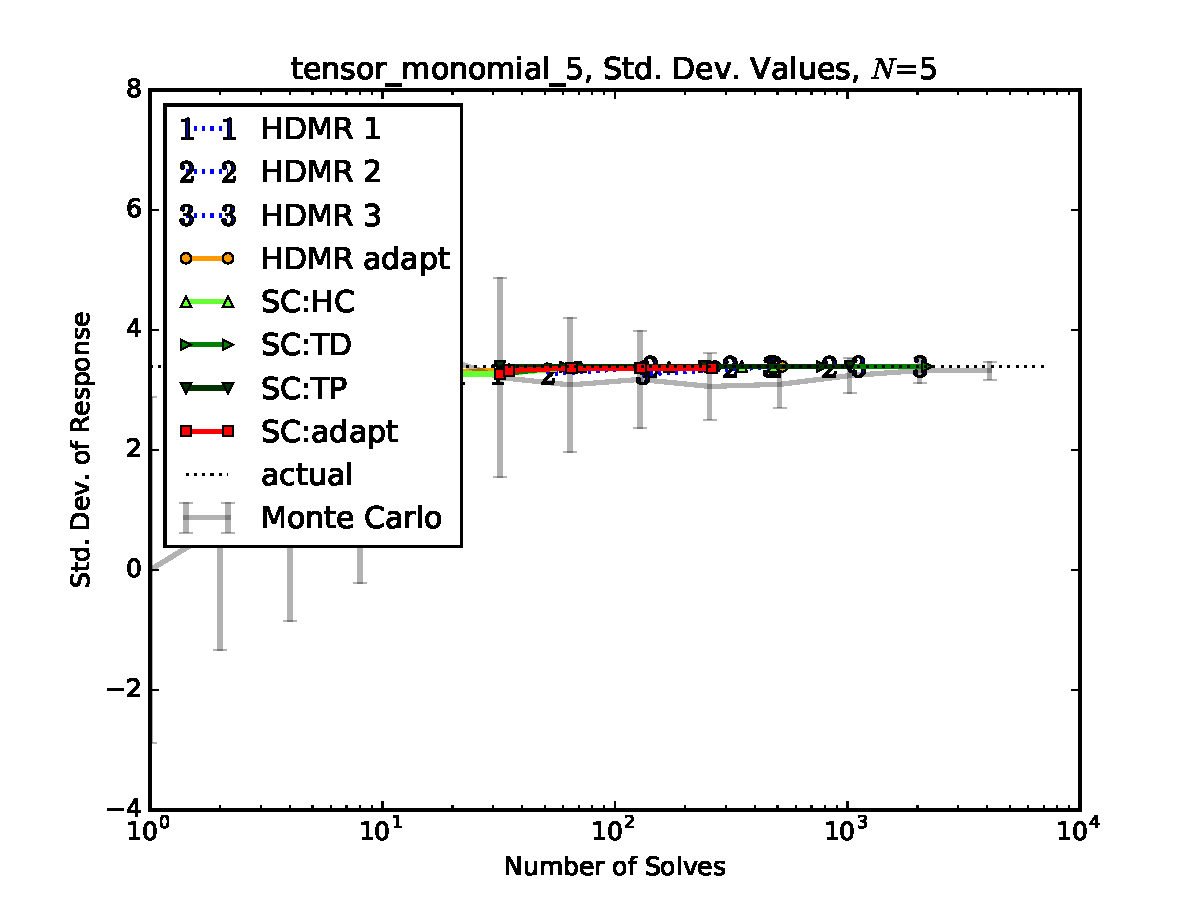
\includegraphics[width=0.7\linewidth]{anlmodels/tensor_monomial_5_var_vals}
  \caption{Tensor Monomial, $N=5$, Std. Dev. Values}
  \label{fig:hdmr tensormono var values 5}
\end{figure}

\begin{figure}[H]
  \centering
  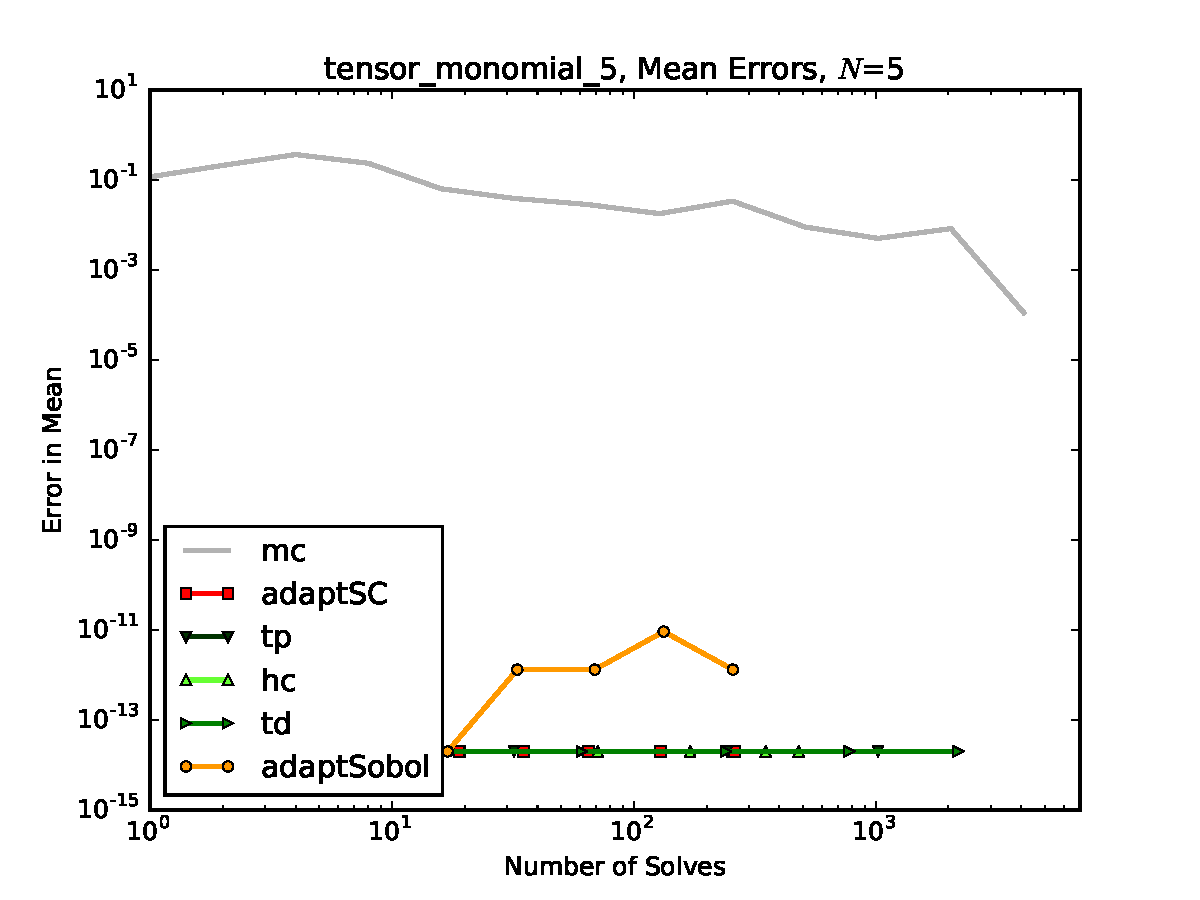
\includegraphics[width=0.7\linewidth]{anlmodels/tensor_monomial_5_mean_errs}
  \caption{Tensor Monomial, $N=5$, Mean Convergence}
  \label{fig:hdmr tensormono mean errors 5}
\end{figure}
\begin{figure}[H]
  \centering
  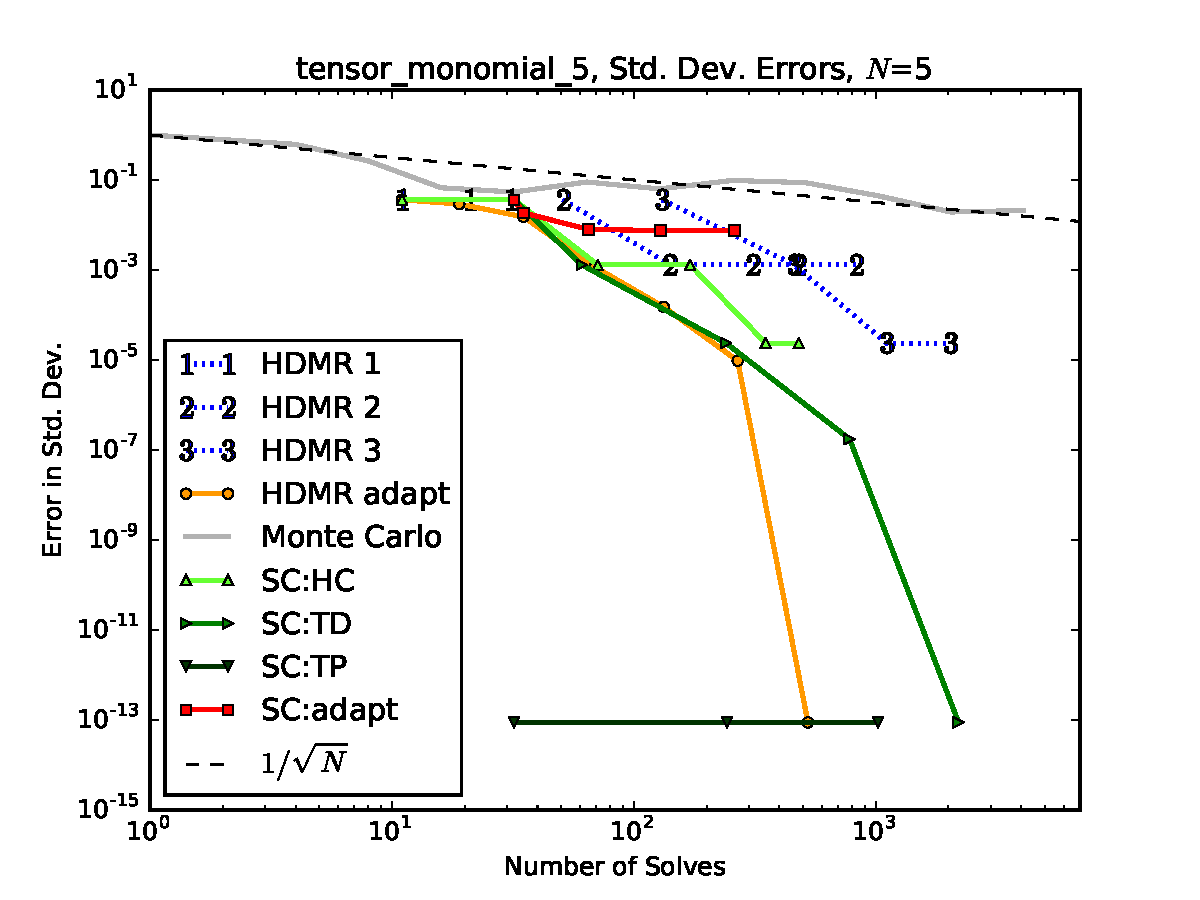
\includegraphics[width=0.7\linewidth]{anlmodels/tensor_monomial_5_variance_errs}
  \caption{Tensor Monomial, $N=5$, Std. Dev. Convergence}
  \label{fig:hdmr tensormono var errors 5}
\end{figure}

\subsection{10 Inputs}
Moving to an input space with dimensionality 10, we predictably see the static HDMR methods performing quite
poorly for this model.  Because the model includes polynomial interactions up to tenth order, truncating at
even three orders incurs significant error.  However, we note the adaptive HDMR method appears to be
performing at least as well as any other method for this larger dimensionality, for the same reasons as
discussed in the 5-input case.  Note also that the adaptive HDMR method obtains representation long before the
total degree or tensor product methods do.
\begin{figure}[H]
  \centering
  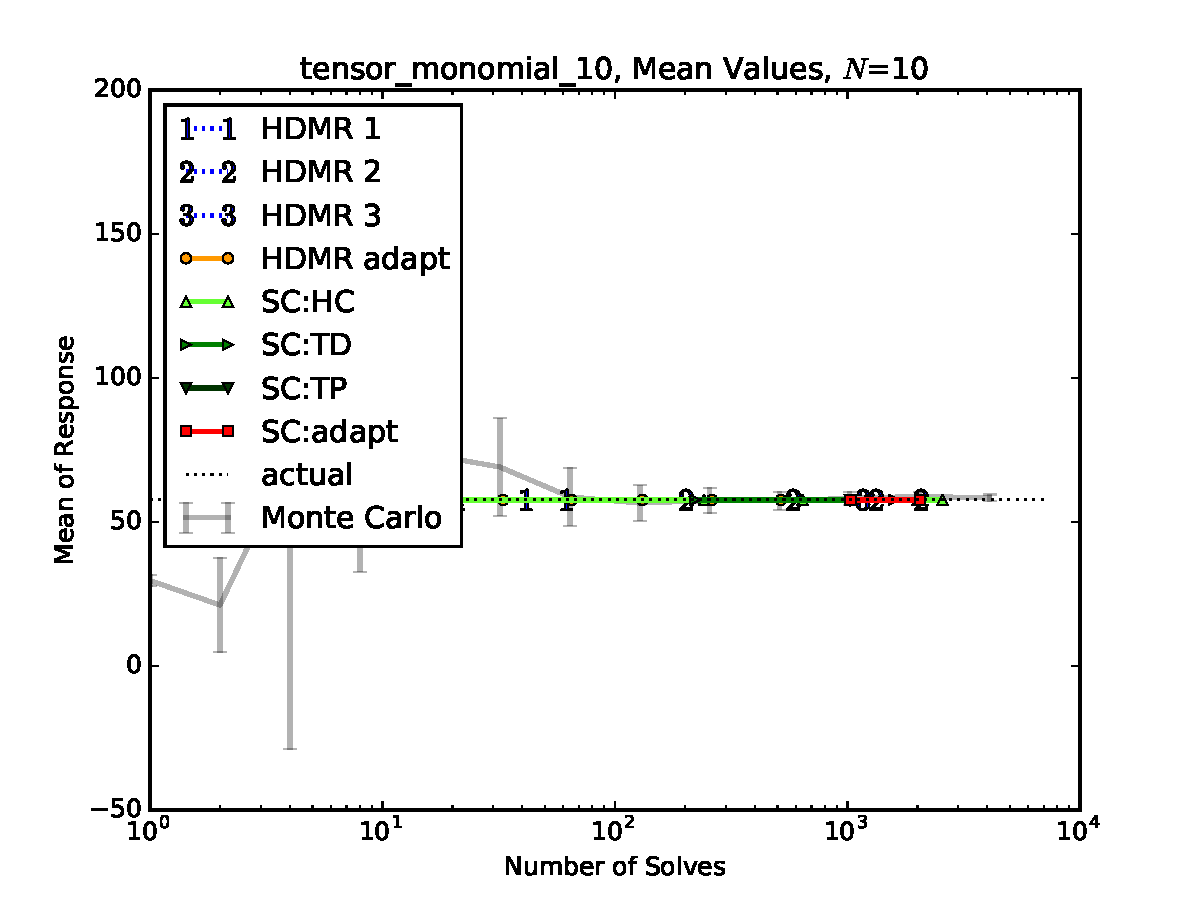
\includegraphics[width=0.7\linewidth]{anlmodels/tensor_monomial_10_mean_vals}
  \caption{Tensor Monomial, $N=10$, Mean Values}
  \label{fig:hdmr tensormono mean values 10}
\end{figure}
\begin{figure}[H]
  \centering
  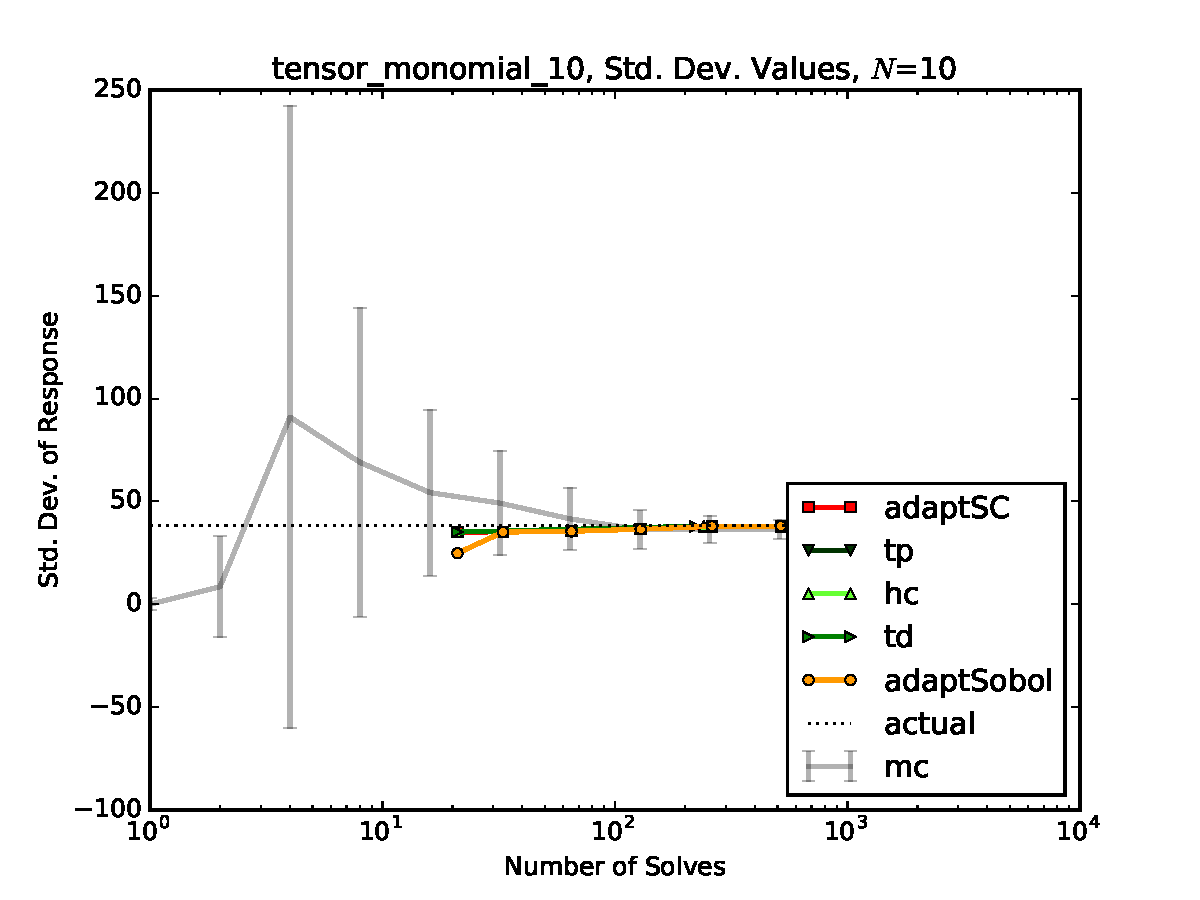
\includegraphics[width=0.7\linewidth]{anlmodels/tensor_monomial_10_var_vals}
  \caption{Tensor Monomial, $N=10$, Std. Dev. Values}
  \label{fig:hdmr tensormono var values 10}
\end{figure}

\begin{figure}[H]
  \centering
  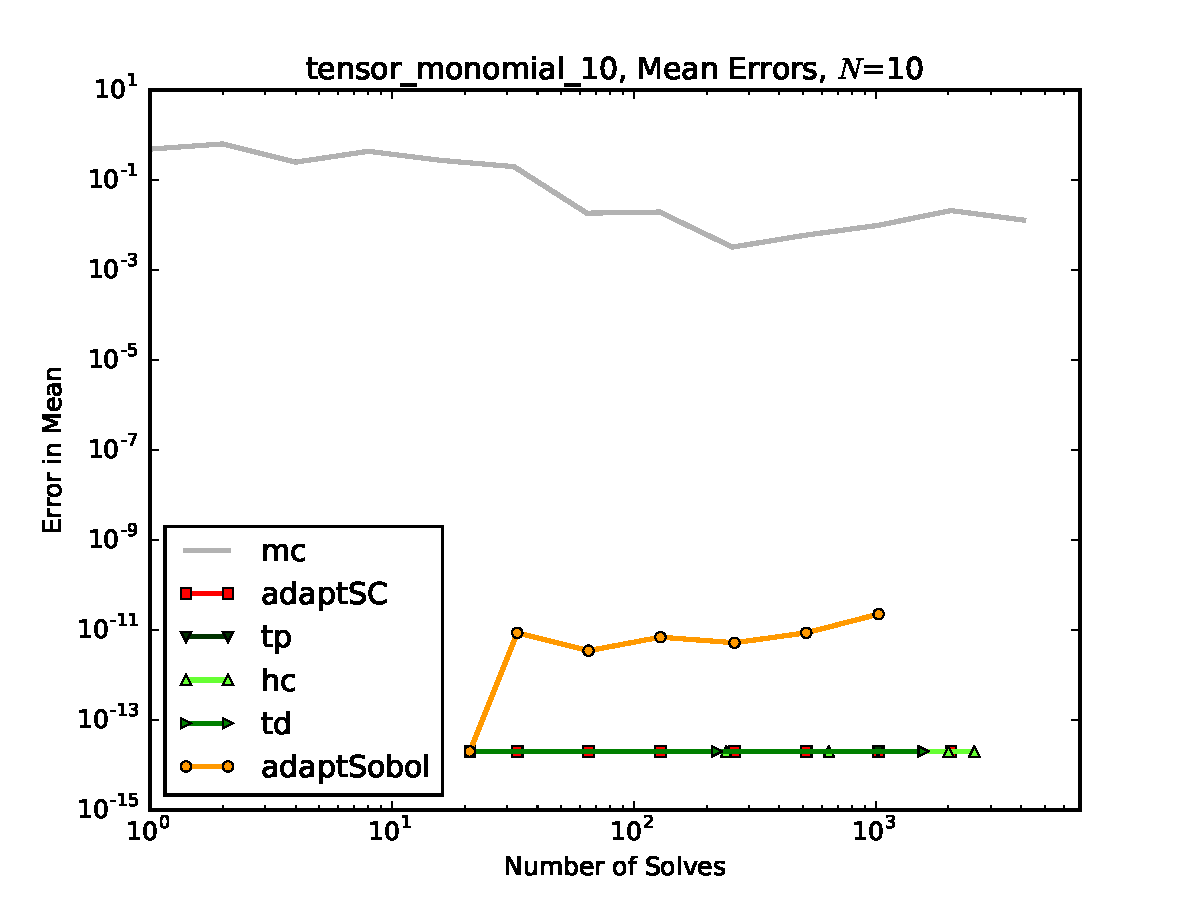
\includegraphics[width=0.7\linewidth]{anlmodels/tensor_monomial_10_mean_errs}
  \caption{Tensor Monomial, $N=10$, Mean Convergence}
  \label{fig:hdmr tensormono mean errors 10}
\end{figure}
\begin{figure}[H]
  \centering
  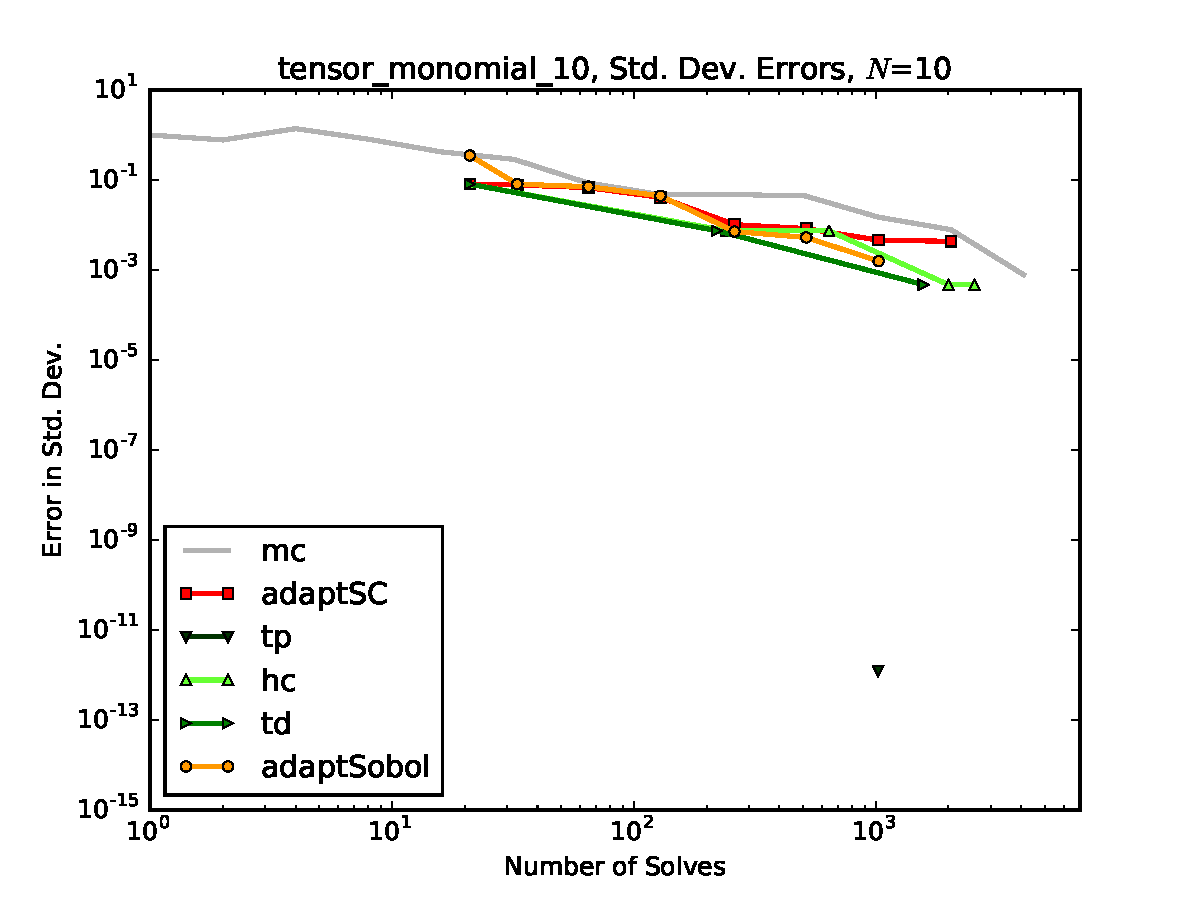
\includegraphics[width=0.7\linewidth]{anlmodels/tensor_monomial_10_variance_errs}
  \caption{Tensor Monomial, $N=10$, Std. Dev. Convergence}
  \label{fig:hdmr tensormono var errors 10}
\end{figure}


\section{Sudret Polynomial}
This model is described in section \ref{mod:sudret}.  This model is similar to the tensor linear polynomials,
but instead is a tensor product of second-order polynomials.  We observe similar performance here as for the
tensor monomials, but with faster degredation as the input dimensionality increases.

\subsection{3 Inputs}
Because of the tensor construction of these polynomials, the HDMR truncation level once again plays a critical
role in determining the error of the HDMR methods.  The three plateaus for HDMR 1, HDMR 2, and HDMR 3 show
that adding higher than second-order polynomials will not substantially decrease the error in these
expansions, indicating that the error is dominated by the HDMR truncation error.  Note also that while the
adaptive HDMR method performs well, it is outperformed by adaptive SCgPC.  This is because it is challenging
for the adaptive HDMR method to find the second-order polynomials while the first-order polynomials have no
contribution to the expansion.  This is especially seen in the convergence of the standard deviation.  Note
that for the standard deviation, HDMR 3 is still converging; this is because the HDMR subsets are expanded in
total degree index sets, which require higher-order polynomial limits to obtain the tensor product of
second-order polynomials; in particular, third-order interaction subsets require total degree order 6 to
obtain the polynomial with orders $k=(2,2,2)$, which is required for this model.
\begin{figure}[H]
  \centering
  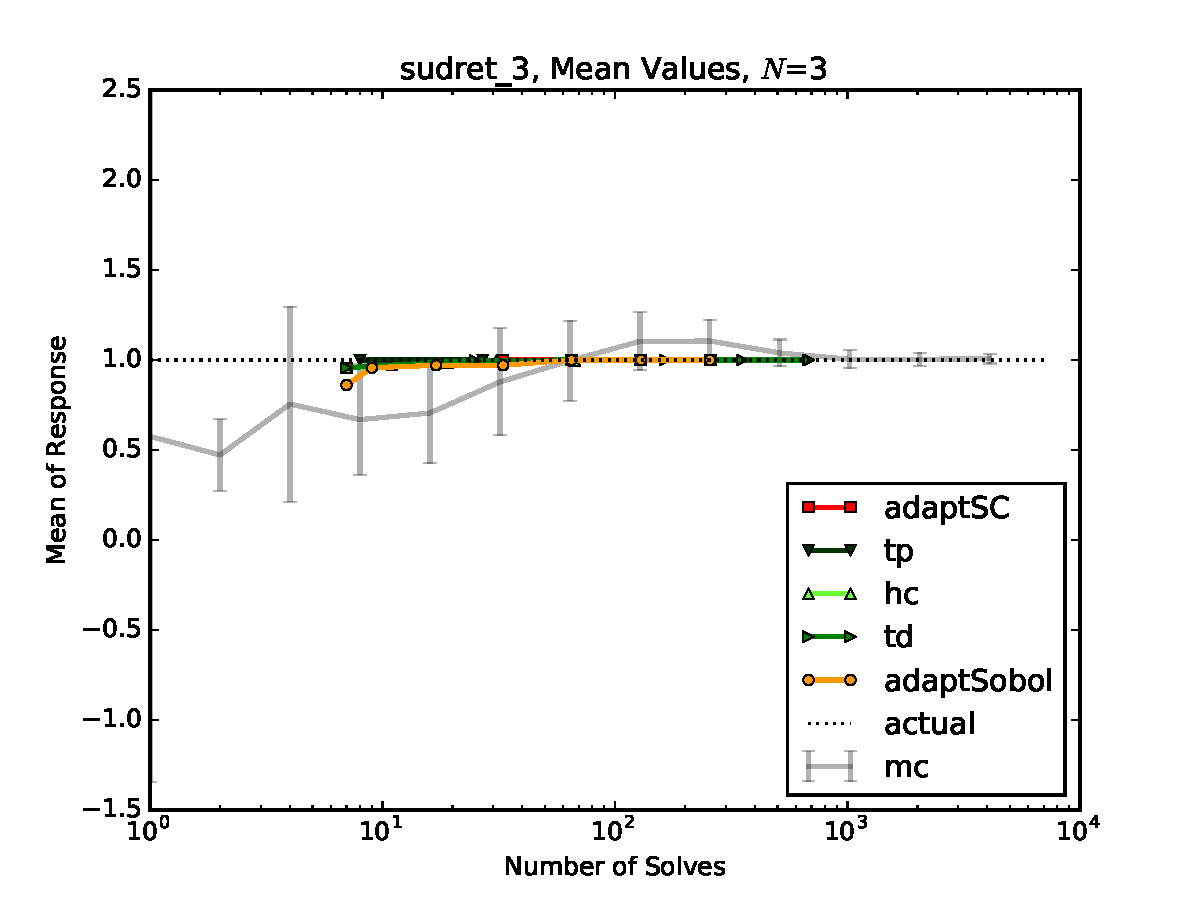
\includegraphics[width=0.7\linewidth]{anlmodels/sudret_3_mean_vals}
  \caption{Sudret Polynomial, $N=3$, Mean Values}
  \label{fig:hdmr sudretpoly mean values 3}
\end{figure}
\begin{figure}[H]
  \centering
  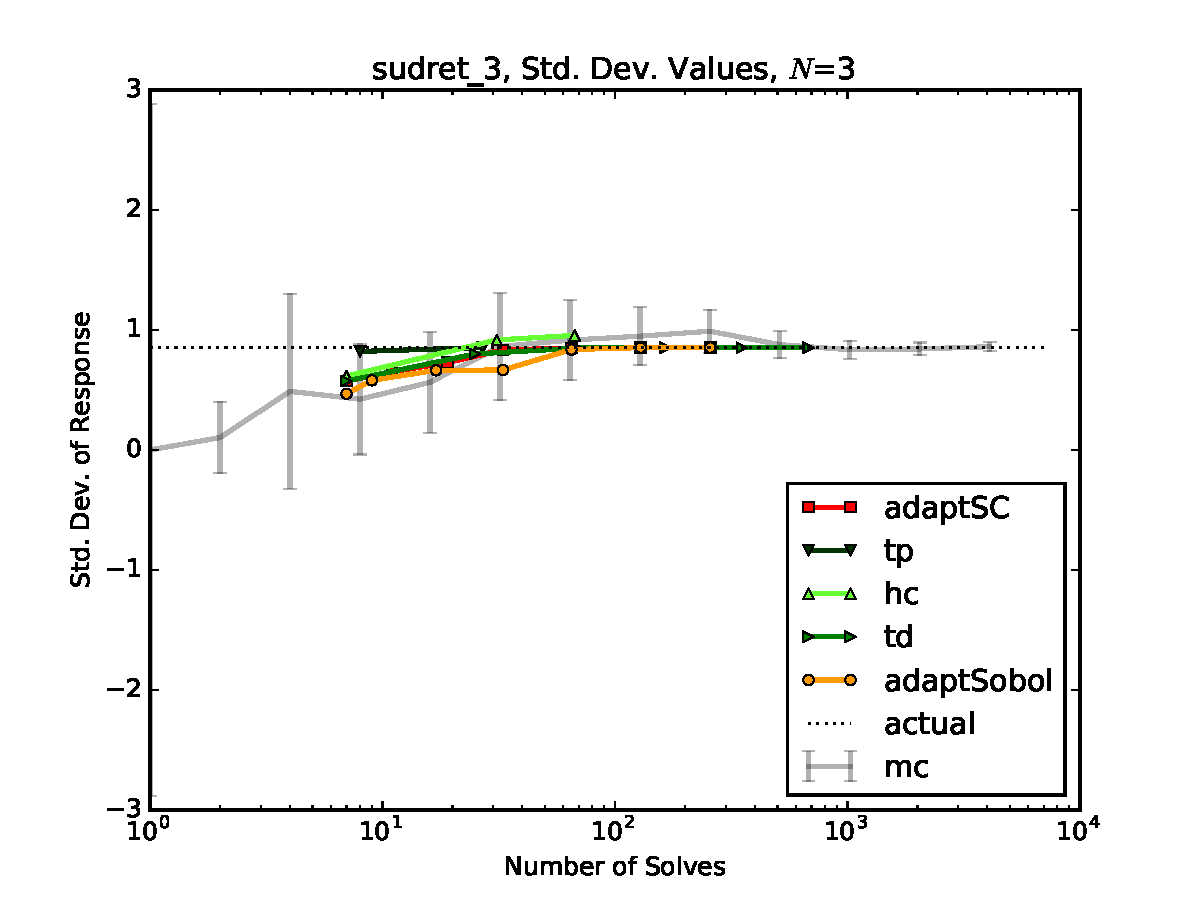
\includegraphics[width=0.7\linewidth]{anlmodels/sudret_3_var_vals}
  \caption{Sudret Polynomial, $N=3$, Std. Dev. Values}
  \label{fig:hdmr sudretpoly var values 3}
\end{figure}

\begin{figure}[H]
  \centering
  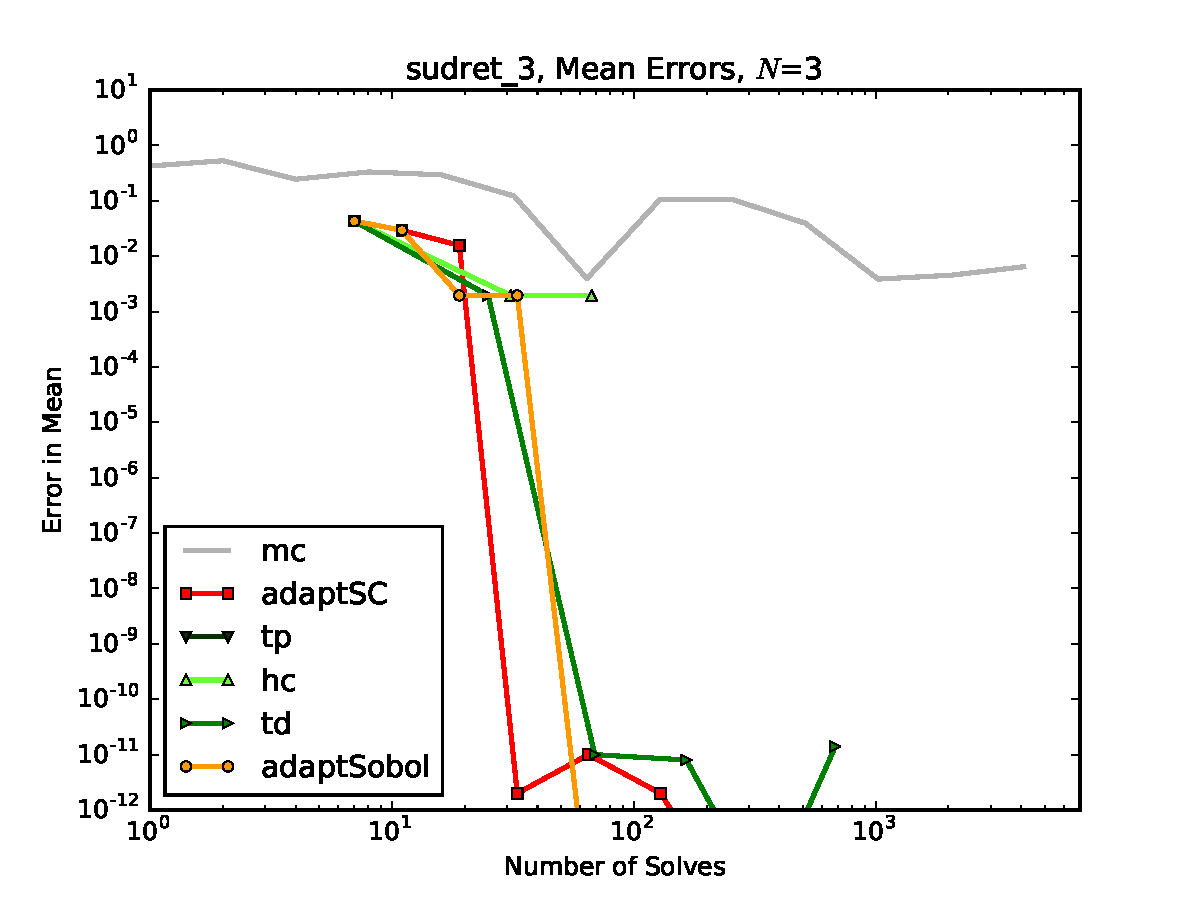
\includegraphics[width=0.7\linewidth]{anlmodels/sudret_3_mean_errs}
  \caption{Sudret Polynomial, $N=3$, Mean Convergence}
  \label{fig:hdmr sudretpoly mean errors 3}
\end{figure}
\begin{figure}[H]
  \centering
  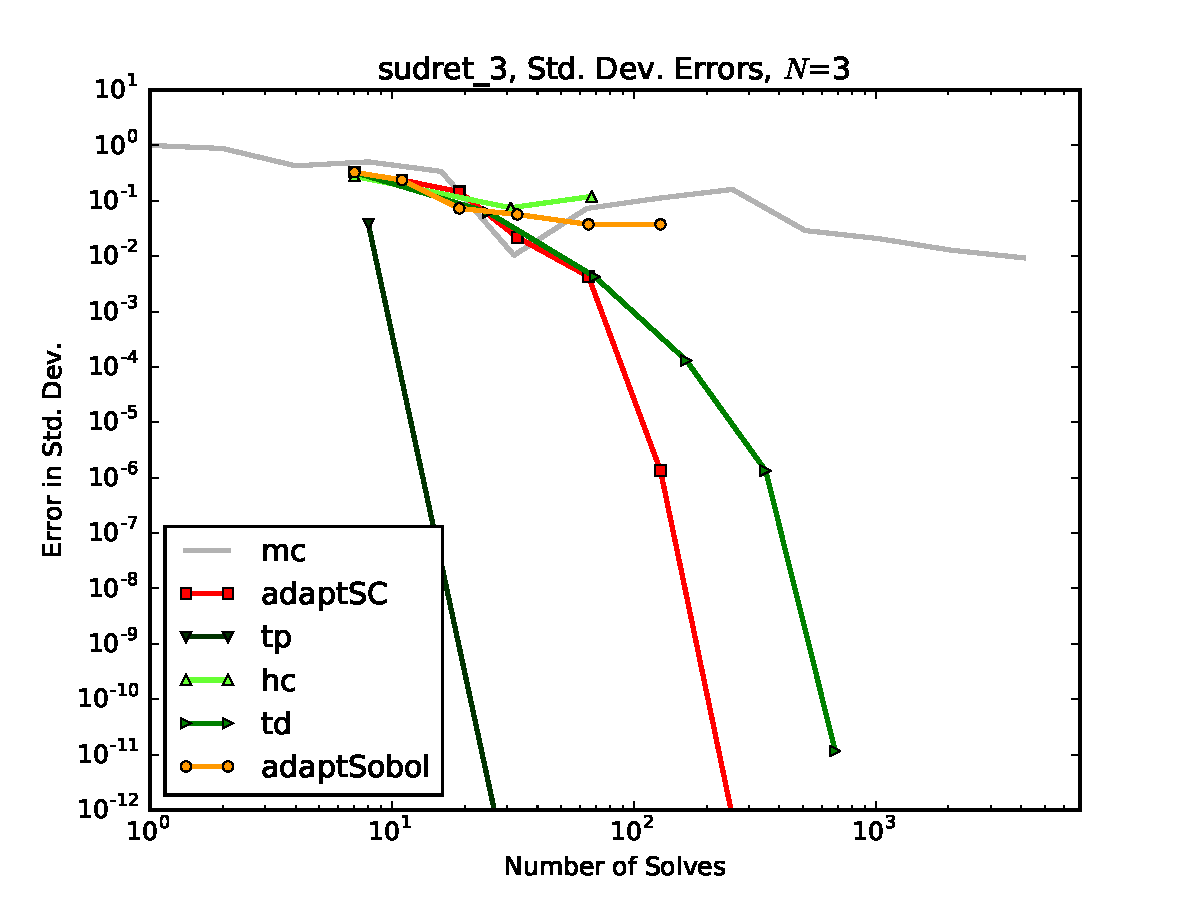
\includegraphics[width=0.7\linewidth]{anlmodels/sudret_3_variance_errs}
  \caption{Sudret Polynomial, $N=3$, Std. Dev. Convergence}
  \label{fig:hdmr sudretpoly var errors 3}
\end{figure}

\subsection{5 Inputs}
We continue to see degredation of performance from HDMR methods moving from three inputs to five.  The
truncation of HDMR 1, HDMR 2, and HDMR 3 incurs too much error to converge significantly, and the adaptive
HDMR method struggles like the adaptive SCgPC method to explore the polynomial space effectively.  
\begin{figure}[H]
  \centering
  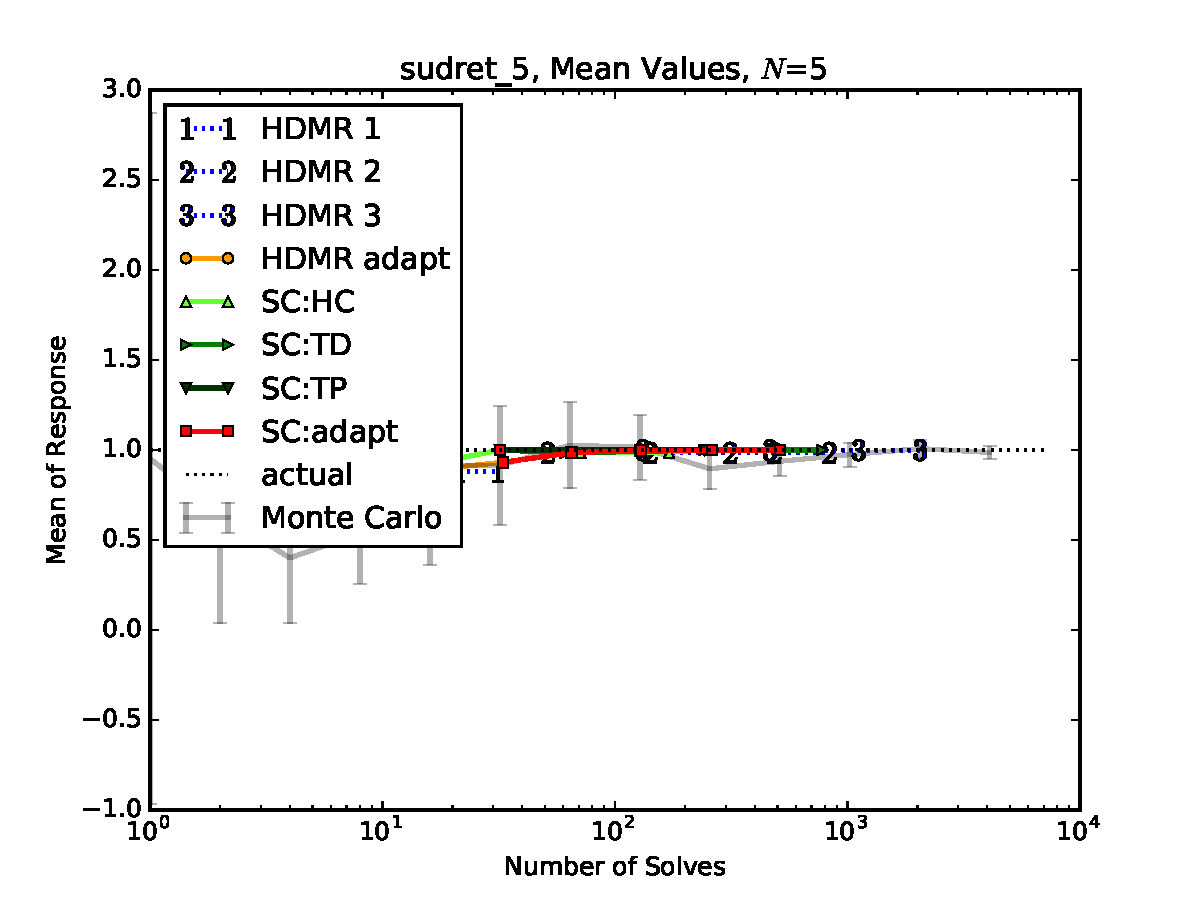
\includegraphics[width=0.7\linewidth]{anlmodels/sudret_5_mean_vals}
  \caption{Sudret Polynomial, $N=5$, Mean Values}
  \label{fig:hdmr sudretpoly mean values 5}
\end{figure}
\begin{figure}[H]
  \centering
  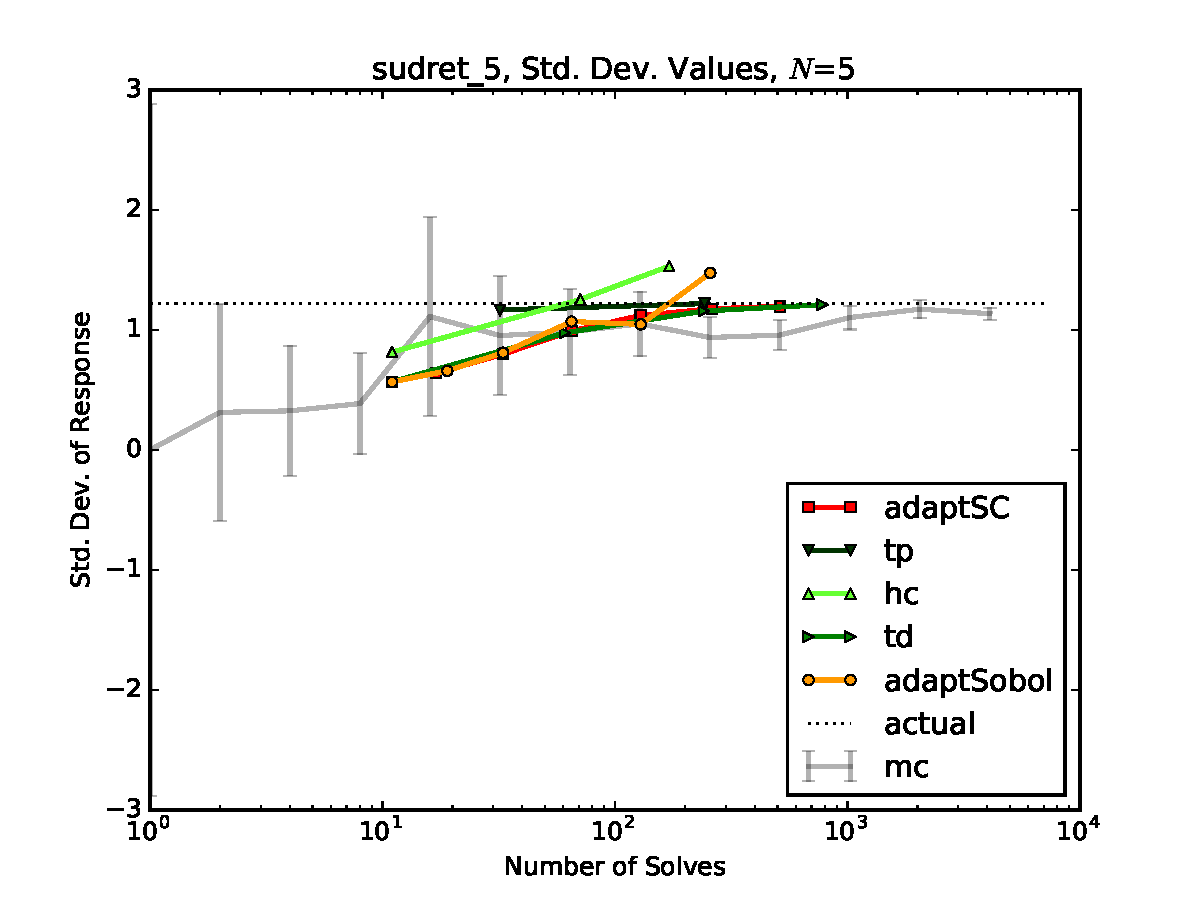
\includegraphics[width=0.7\linewidth]{anlmodels/sudret_5_var_vals}
  \caption{Sudret Polynomial, $N=5$, Std. Dev. Values}
  \label{fig:hdmr sudretpoly var values 5}
\end{figure}

\begin{figure}[H]
  \centering
  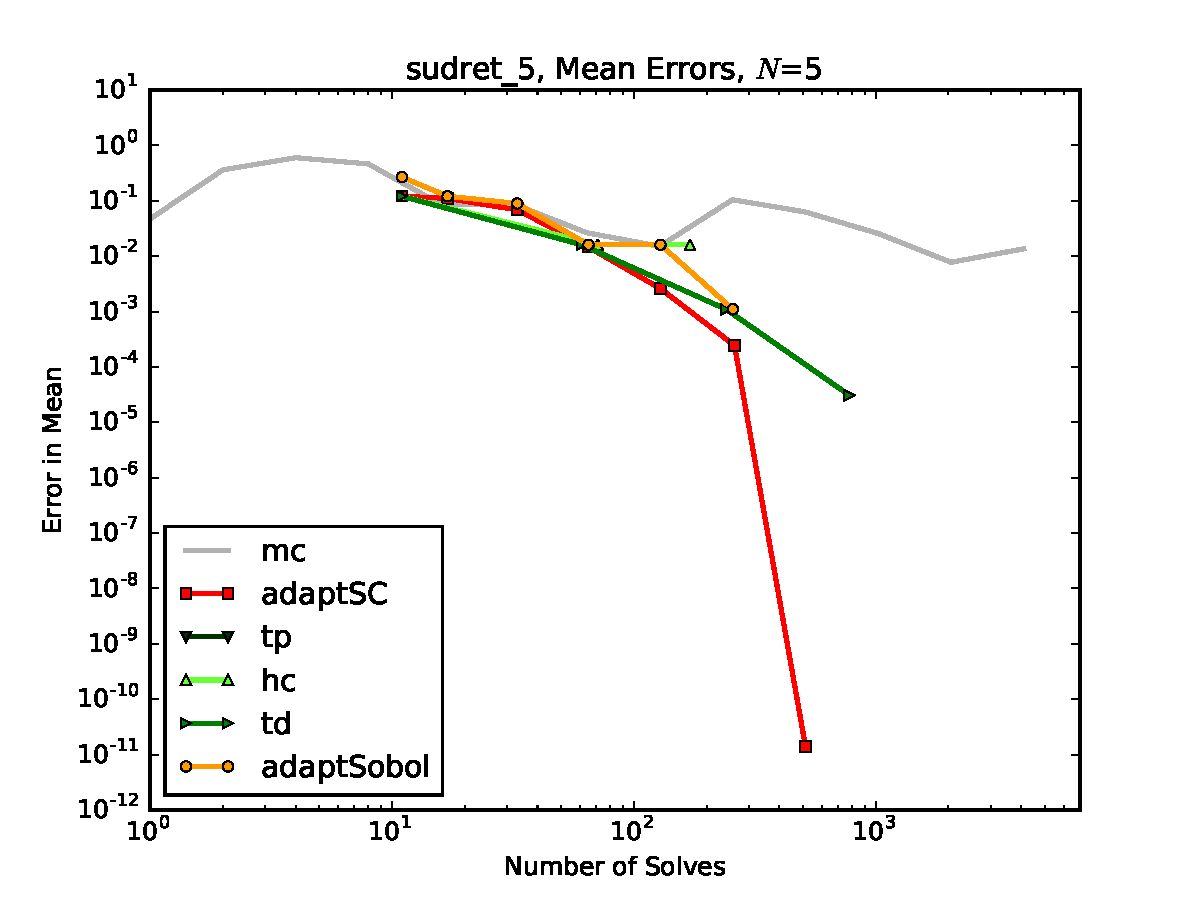
\includegraphics[width=0.7\linewidth]{anlmodels/sudret_5_mean_errs}
  \caption{Sudret Polynomial, $N=5$, Mean Convergence}
  \label{fig:hdmr sudretpoly mean errors 5}
\end{figure}
\begin{figure}[H]
  \centering
  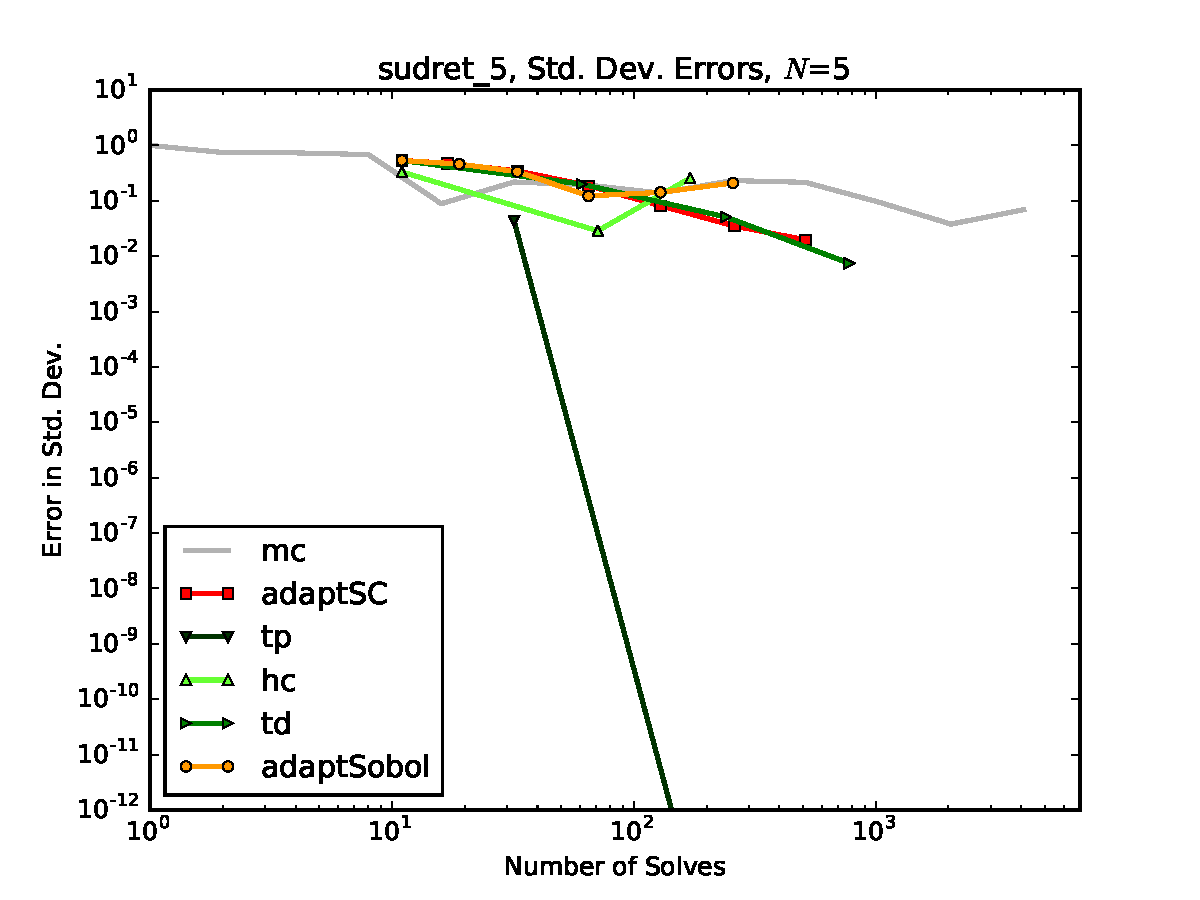
\includegraphics[width=0.7\linewidth]{anlmodels/sudret_5_variance_errs}
  \caption{Sudret Polynomial, $N=5$, Std. Dev. Convergence}
  \label{fig:hdmr sudretpoly var errors 5}
\end{figure}


\section{Attenuation}
This model is described in section \ref{mod:attenuation}.  As the tensor product of polynomials whose scaling
drops off with increasing order (see Table \ref{tab:atten coeffs}), this model is well-suited to HDMR methods.
However, this model demonstrates some of the limitations in the default search parameters for the adaptive
HDMR method.  While combinations of polynomials of similar order are most important to this expansion, the
adaptive HDMR method tends to expand polynomials with low interaction because of the sensitivity estimation
methods.  This demonstrates when the adaptive HDMR might be ill-suited to exploring the input space.

\subsection{2 Inputs}
Because the input space is only two-dimensional, HDMR 3 is equivalent to HDMR 2 and not shown in this case.
As with the SCgPC methods, all HDMR methods show exponential convergence on the mean and standard deviation
for this response, although the adaptive HDMR does not perform as well as the adaptive SCgPC method because of
the way the polynomial coefficients decay.  The HDMR 1 method stagnates at first-order interactions, and
error is dominated by the HDMR truncation instead of polynomial truncation.
\begin{figure}[H]
  \centering
  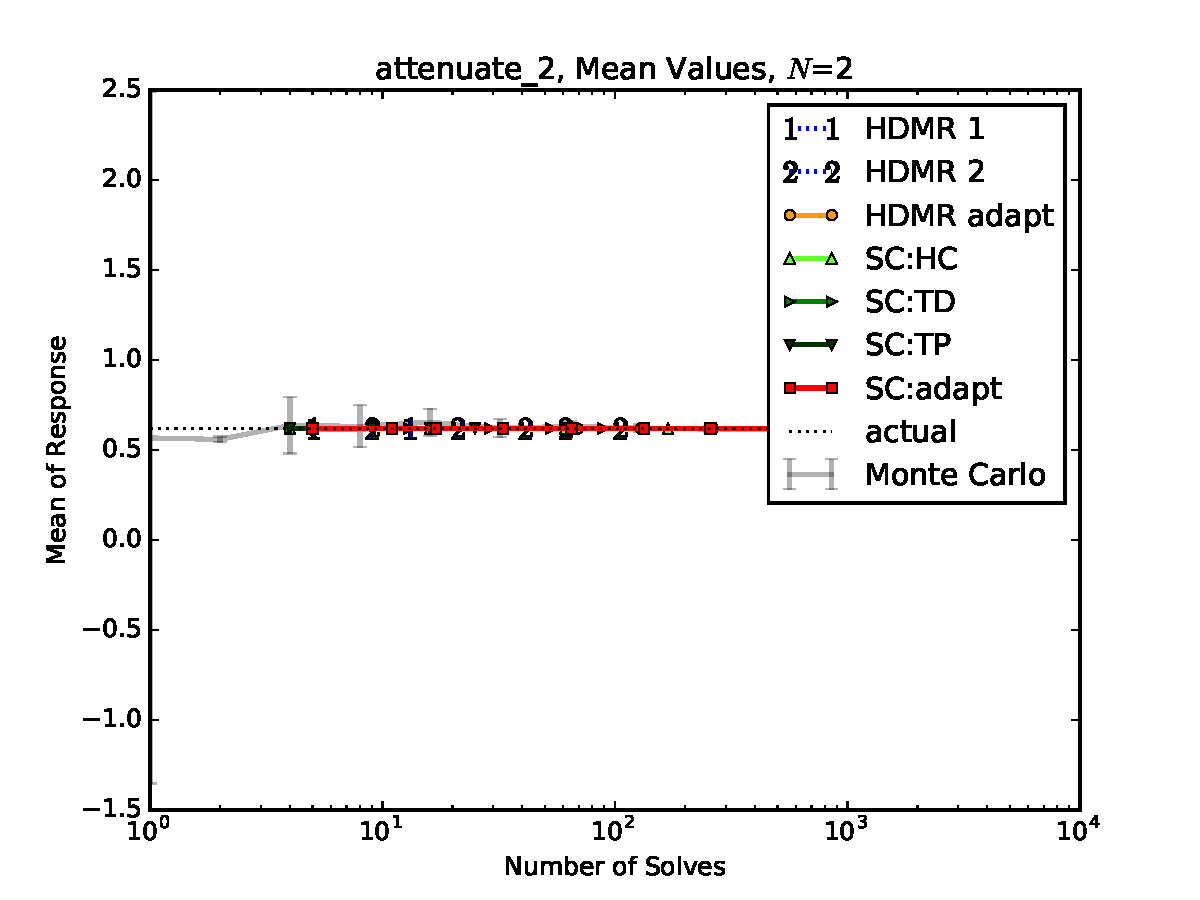
\includegraphics[width=0.7\linewidth]{anlmodels/attenuate_2_mean_vals}
  \caption{Attenuation, $N=2$, Mean Values}
  \label{fig:hdmr attenuate mean values 2}
\end{figure}
\begin{figure}[H]
  \centering
  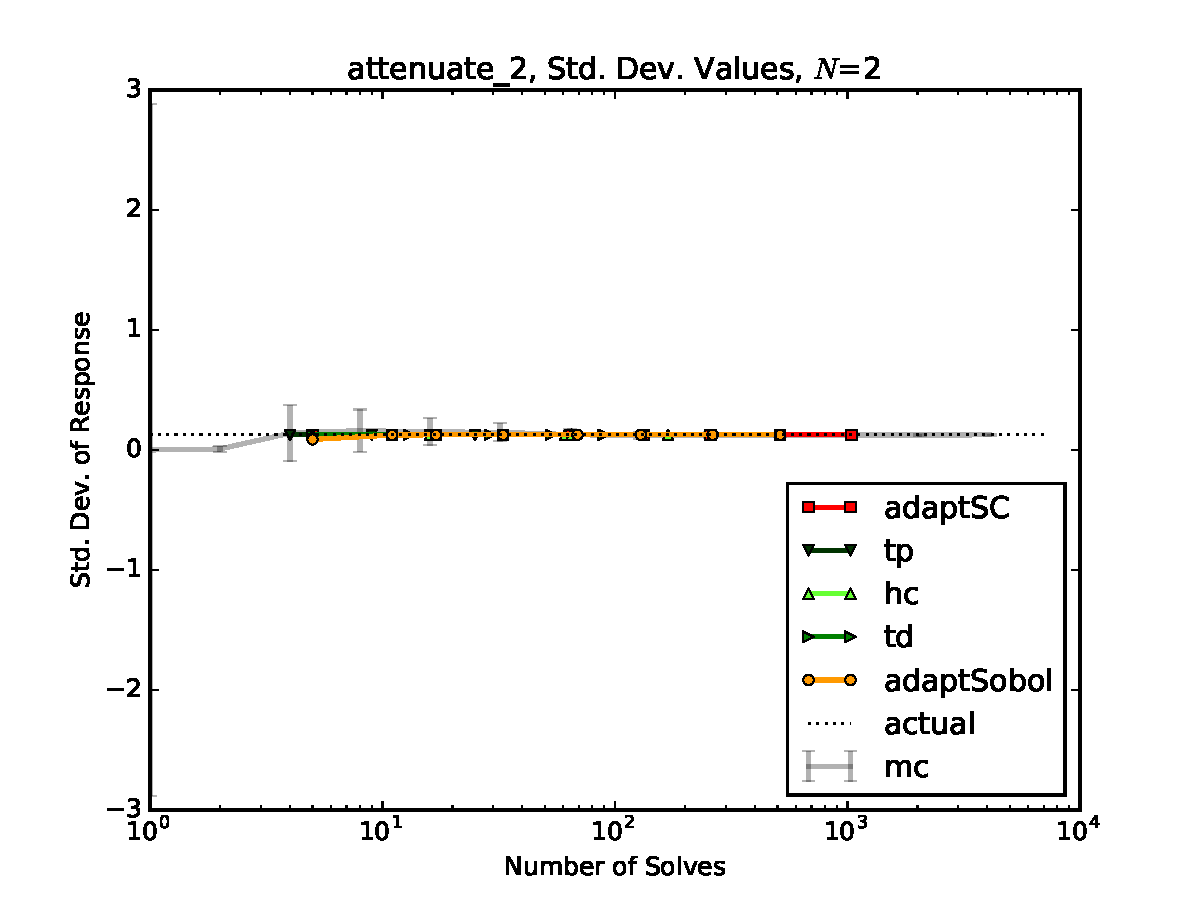
\includegraphics[width=0.7\linewidth]{anlmodels/attenuate_2_var_vals}
  \caption{Attenuation, $N=2$, Std. Dev. Values}
  \label{fig:hdmr attenuate var values 2}
\end{figure}

\begin{figure}[H]
  \centering
  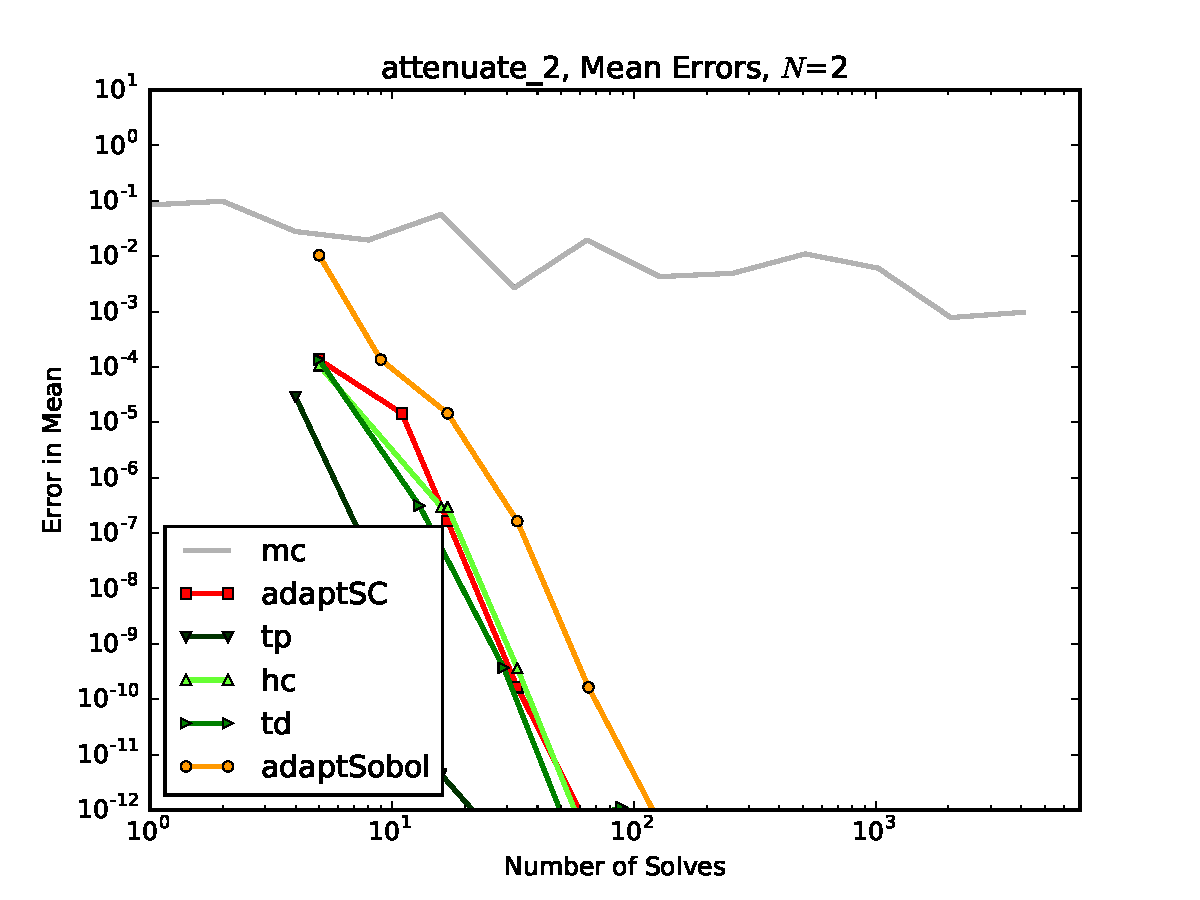
\includegraphics[width=0.7\linewidth]{anlmodels/attenuate_2_mean_errs}
  \caption{Attenuation, $N=2$, Mean Convergence}
  \label{fig:hdmr attenuate mean errors 2}
\end{figure}
\begin{figure}[H]
  \centering
  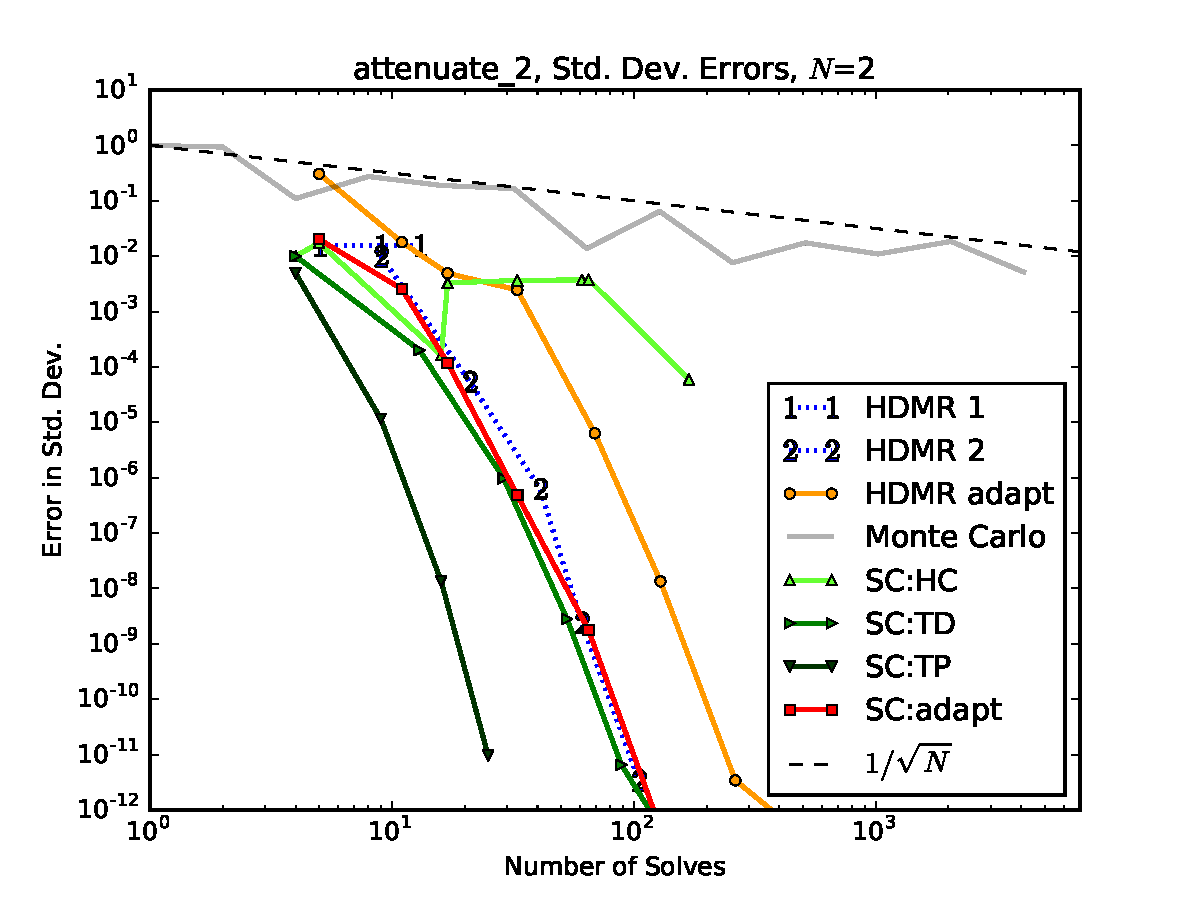
\includegraphics[width=0.7\linewidth]{anlmodels/attenuate_2_variance_errs}
  \caption{Attenuation, $N=2$, Std. Dev. Convergence}
  \label{fig:hdmr attenuate var errors 2}
\end{figure}


\subsection{4 Inputs}
The same trends exist here as for the two-dimensional case, but with degradation because of the increase in
dimensionality.  The plateaus for HDMR 1, HDMR 2, and HDMR 3 are all clearly evident.  These plateaus indicate
when error is dominated by HDMR truncation instead of polynomial truncation.  It is also worth noting that
while the adaptive HDMR method hits a plateau for some time in this model, it obtains a decent approximation
of the standard deviation and mean earlier than most of the other static methods.
\begin{figure}[H]
  \centering
  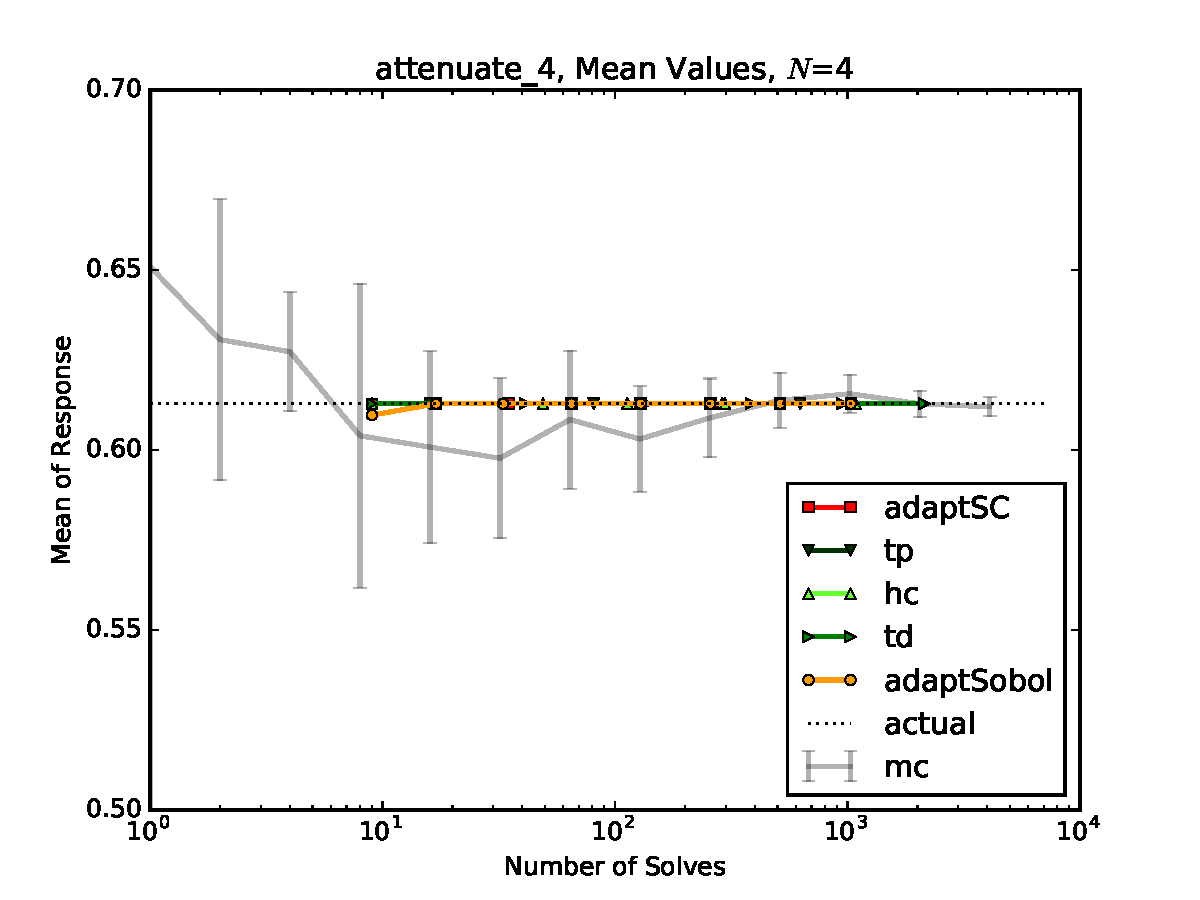
\includegraphics[width=0.7\linewidth]{anlmodels/attenuate_4_mean_vals}
  \caption{Attenuation, $N=4$, Mean Values}
  \label{fig:hdmr attenuate mean values 4}
\end{figure}
\begin{figure}[H]
  \centering
  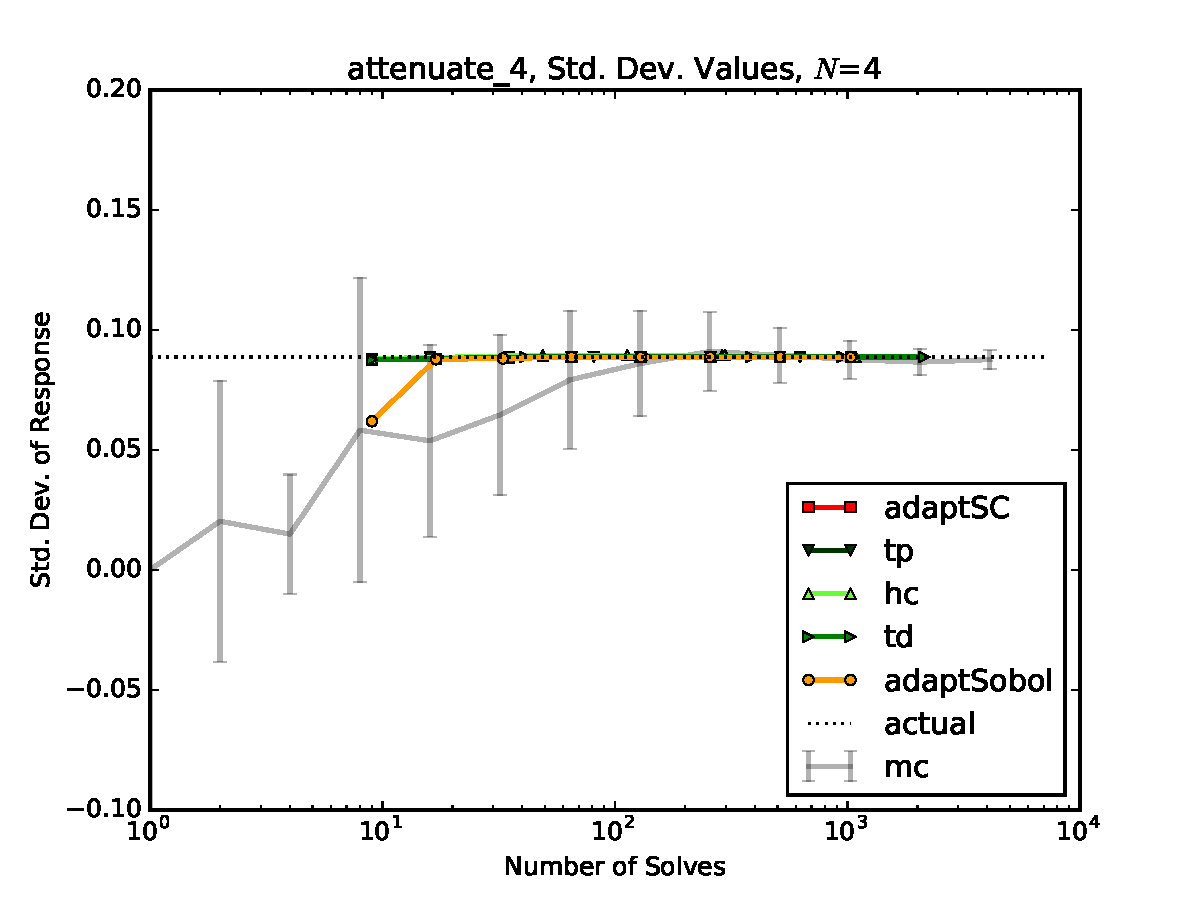
\includegraphics[width=0.7\linewidth]{anlmodels/attenuate_4_var_vals}
  \caption{Attenuation, $N=4$, Std. Dev. Values}
  \label{fig:hdmr attenuate var values 4}
\end{figure}

\begin{figure}[H]
  \centering
  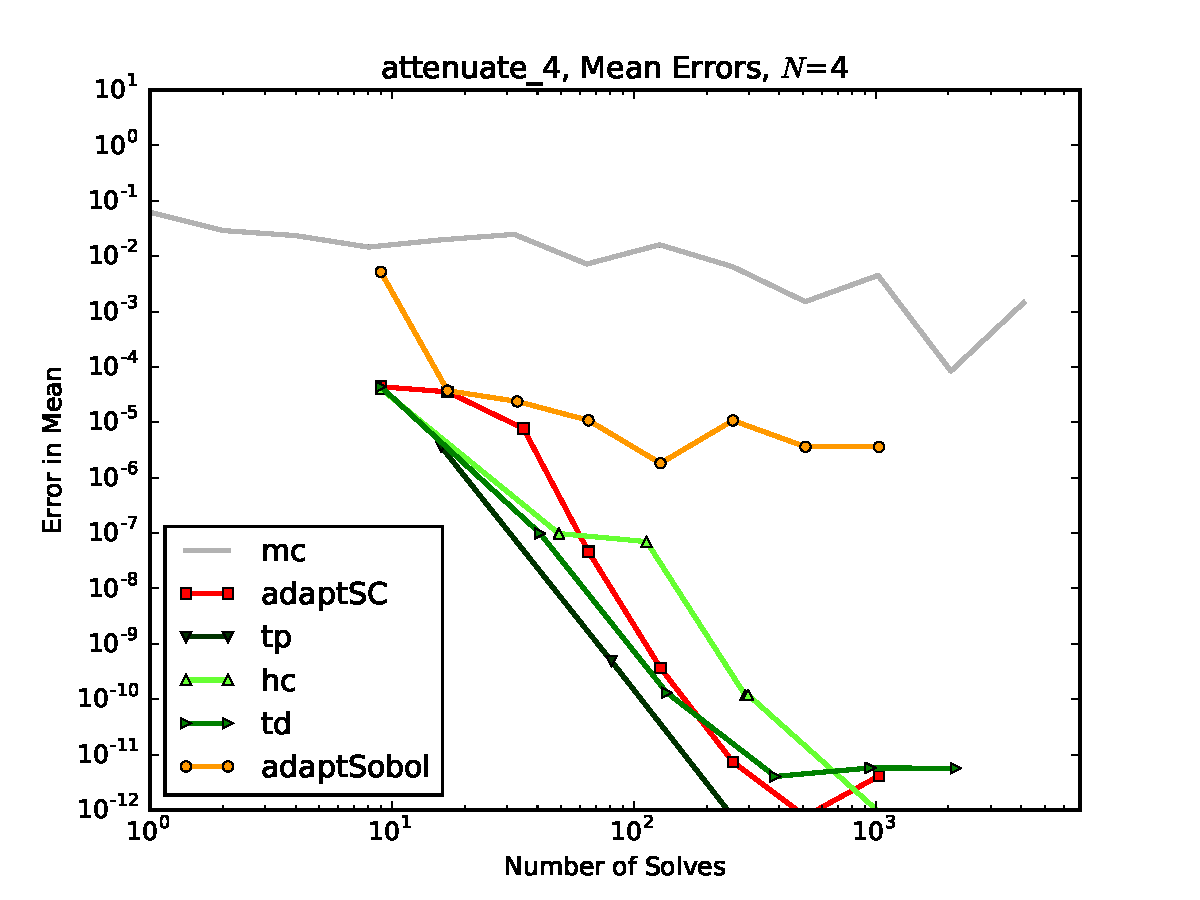
\includegraphics[width=0.7\linewidth]{anlmodels/attenuate_4_mean_errs}
  \caption{Attenuation, $N=4$, Mean Convergence}
  \label{fig:hdmr attenuate mean errors 4}
\end{figure}
\begin{figure}[H]
  \centering
  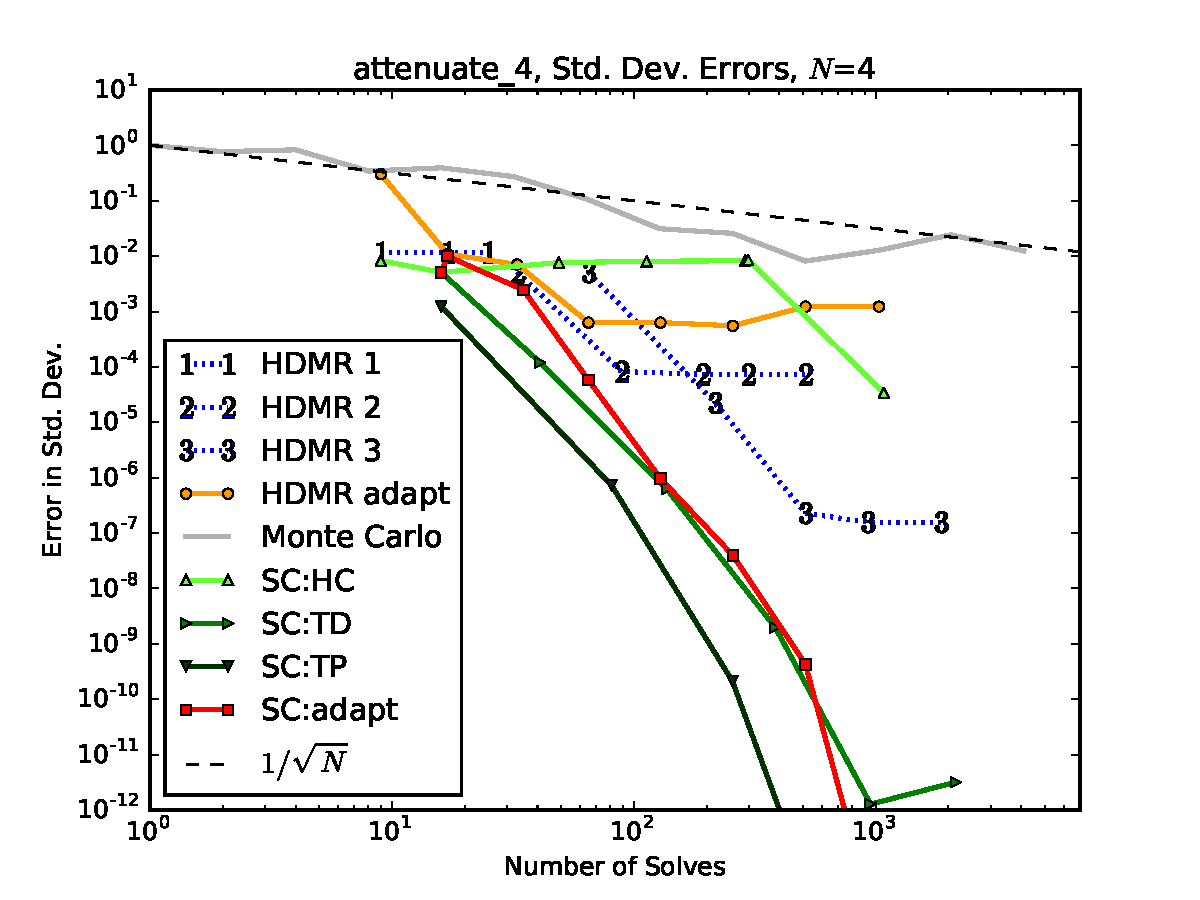
\includegraphics[width=0.7\linewidth]{anlmodels/attenuate_4_variance_errs}
  \caption{Attenuation, $N=4$, Std. Dev. Convergence}
  \label{fig:hdmr attenuate var errors 4}
\end{figure}

\subsection{6 Inputs}
The SCgPC and HDMR methods continue to degrade as input space increases in dimensionality.  The static method
plateaus are still evident.  The adaptive SCgPC and adaptive HDMR methods both struggle to find the
appropriate polynomials to use to most accurately represent this model.
\begin{figure}[H]
  \centering
  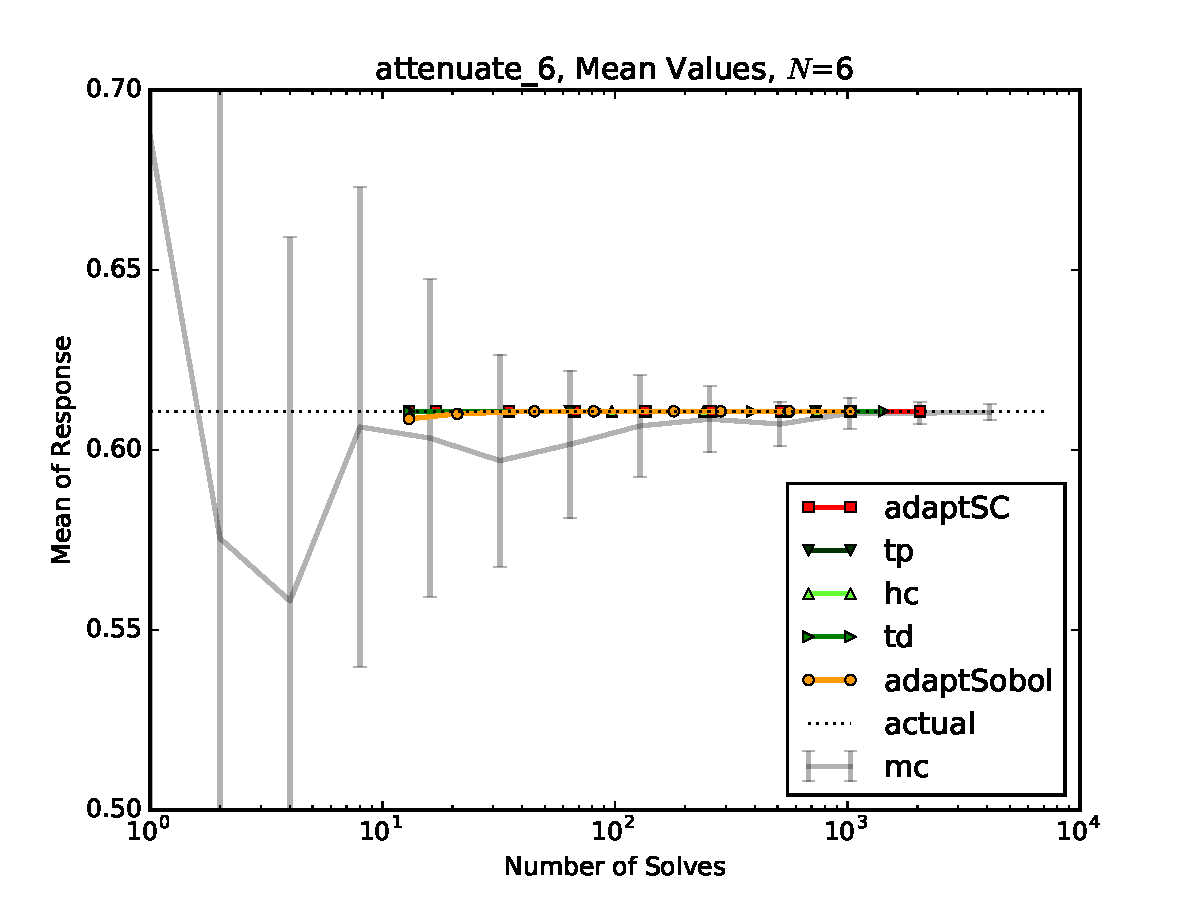
\includegraphics[width=0.7\linewidth]{anlmodels/attenuate_6_mean_vals}
  \caption{Attenuation, $N=6$, Mean Values}
  \label{fig:hdmr attenuate mean values 6}
\end{figure}
\begin{figure}[H]
  \centering
  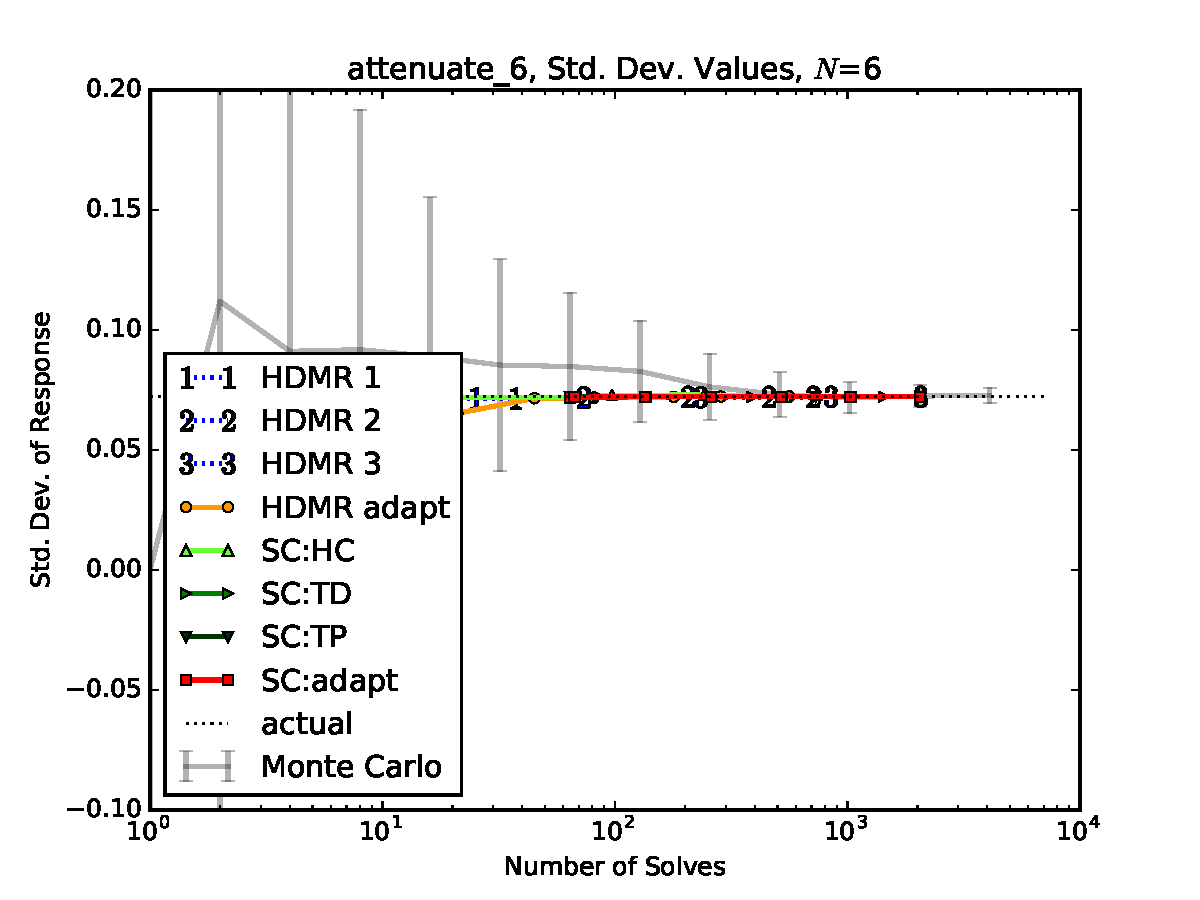
\includegraphics[width=0.7\linewidth]{anlmodels/attenuate_6_var_vals}
  \caption{Attenuation, $N=6$, Std. Dev. Values}
  \label{fig:hdmr attenuate var values 6}
\end{figure}

\begin{figure}[H]
  \centering
  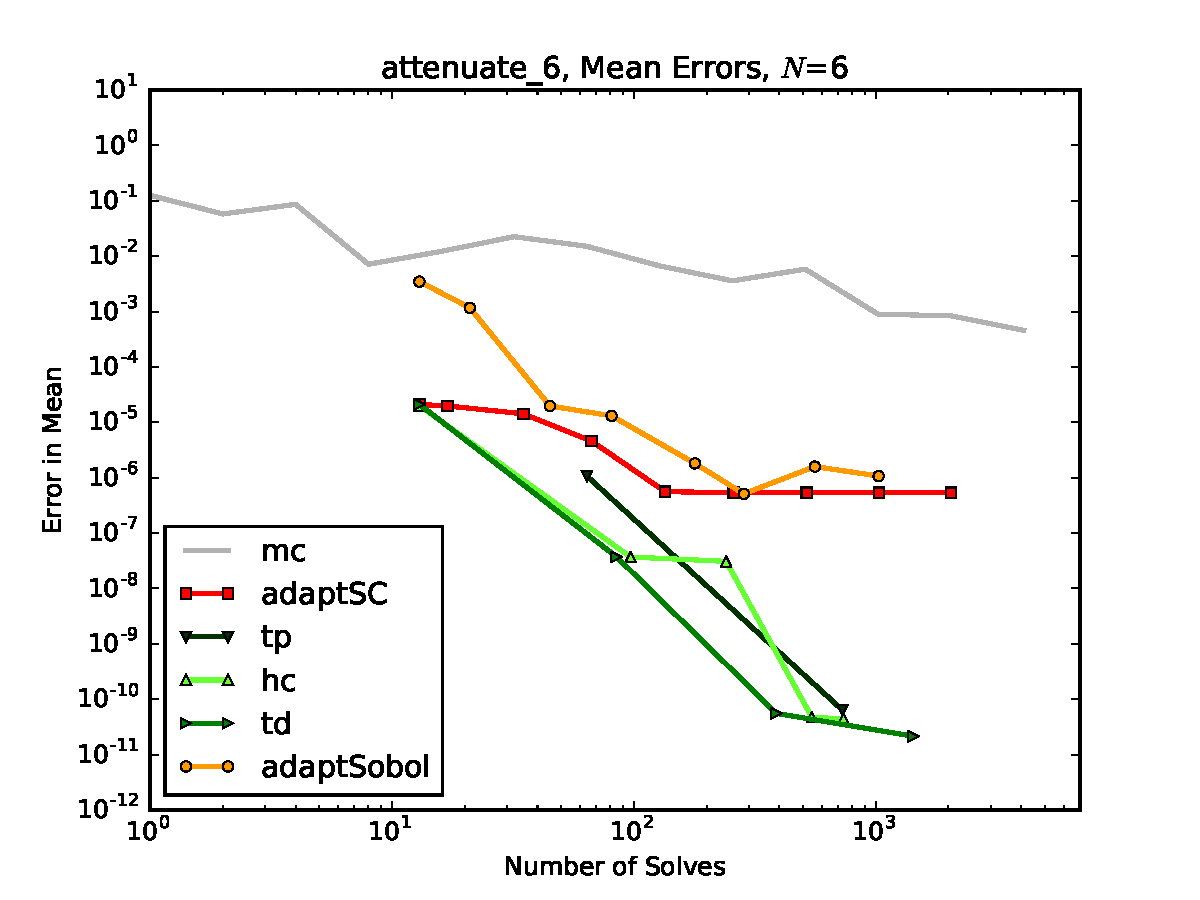
\includegraphics[width=0.7\linewidth]{anlmodels/attenuate_6_mean_errs}
  \caption{Attenuation, $N=6$, Mean Convergence}
  \label{fig:hdmr attenuate mean errors 6}
\end{figure}
\begin{figure}[H]
  \centering
  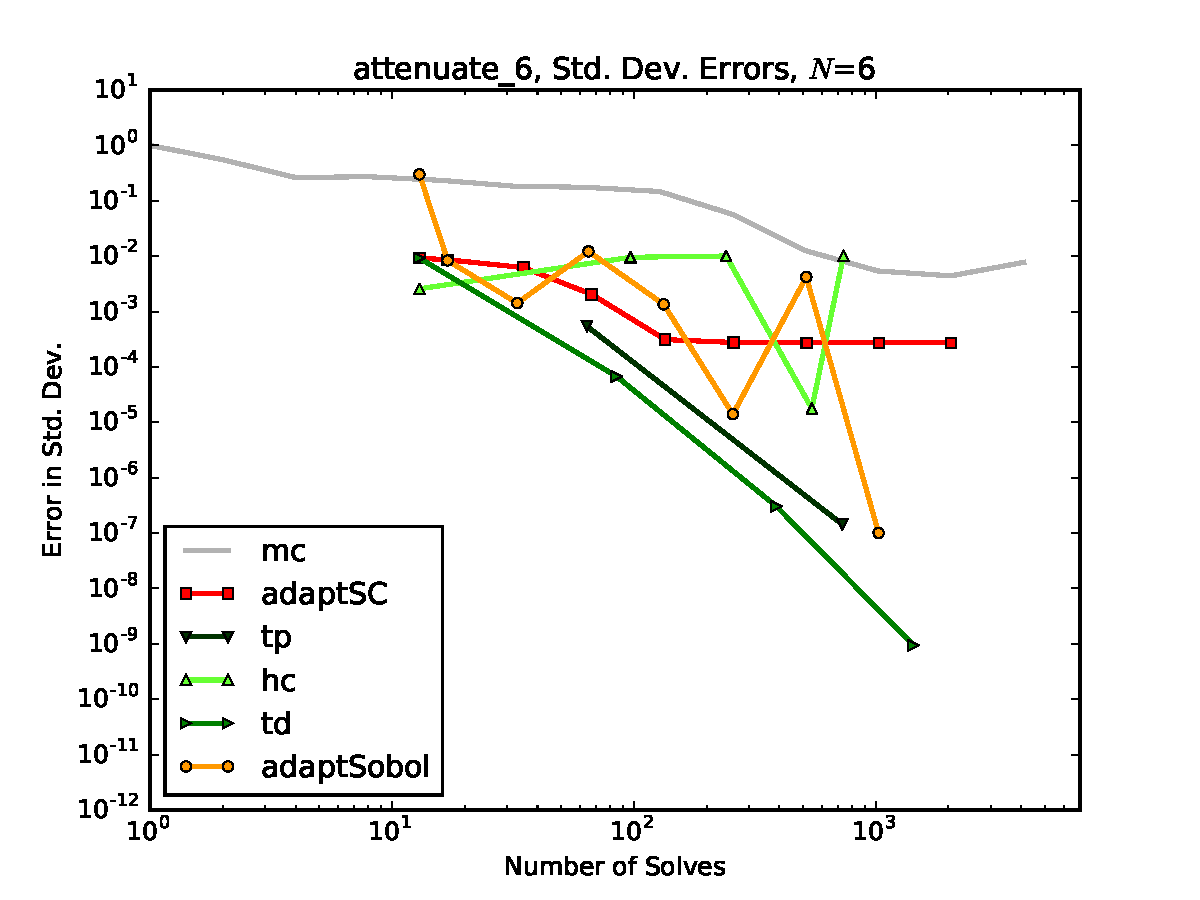
\includegraphics[width=0.7\linewidth]{anlmodels/attenuate_6_variance_errs}
  \caption{Attenuation, $N=6$, Std. Dev. Convergence}
  \label{fig:hdmr attenuate var errors 6}
\end{figure}


\section{Gauss Peak}
This model is described in section \ref{mod:gausspeak}.
As discussed there, this model exhibits slow polynomial coefficient drop off, and all polynomials containing
an odd number have a zero coefficient.  This yields the adaptive search algorithms paralyzed, as any attempts
the assumption of monotonically-decreasing polynomial coefficients is a poor assumption for this model.
\subsection{3 Inputs}
The static HDMR methods show no improvement over Monte Carlo for this model.  It
requires a great number of polynomials in tensor combination to accurately reproduce this response; as a
result, even HDMR 3 shows poor convergence for this model.
\begin{figure}[H]
  \centering
  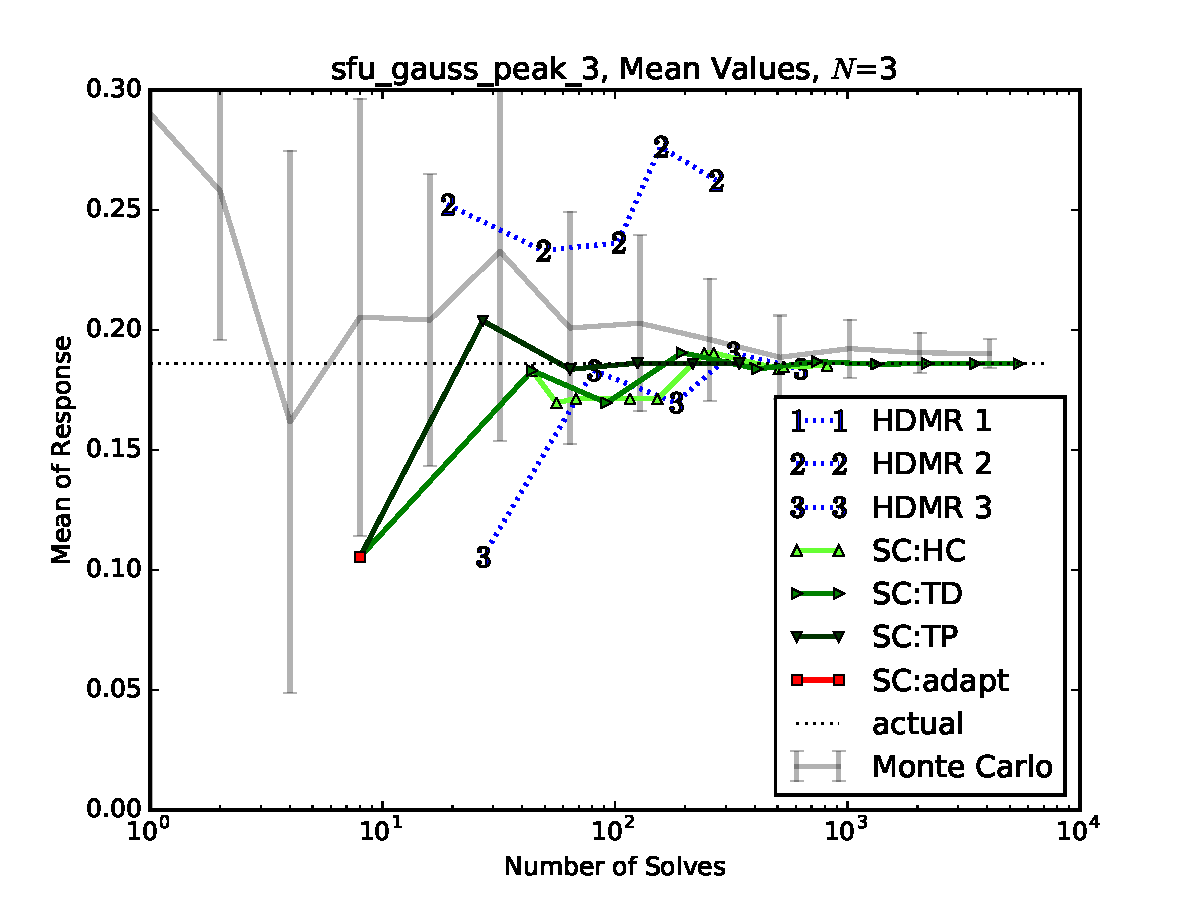
\includegraphics[width=0.7\linewidth]{anlmodels/sfu_gauss_peak_3_mean_vals}
  \caption{Gauss Peak, $N=3$, Mean Values}
  \label{fig:hdmr gauss peak mean values 3}
\end{figure}
\begin{figure}[H]
  \centering
  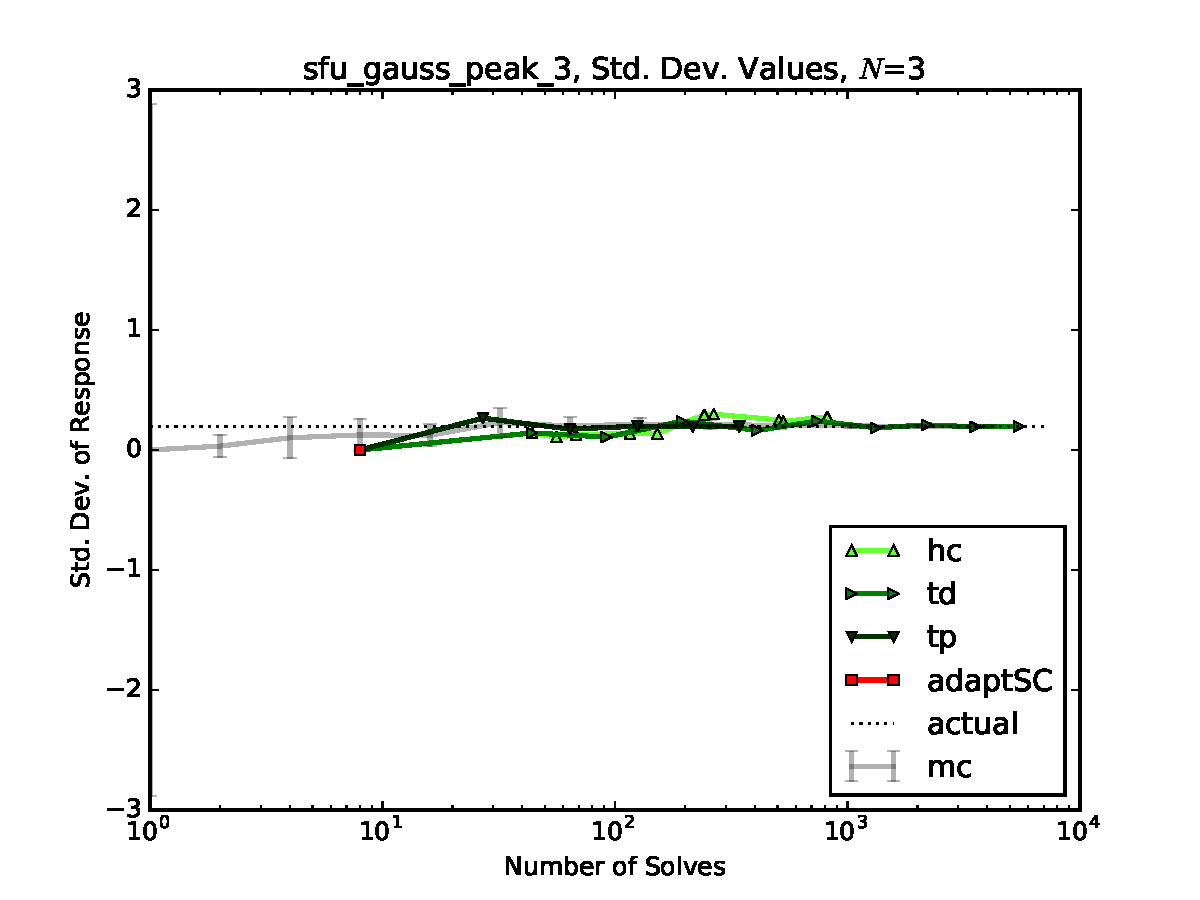
\includegraphics[width=0.7\linewidth]{anlmodels/sfu_gauss_peak_3_var_vals}
  \caption{Gauss Peak, $N=3$, Std. Dev. Values}
  \label{fig:hdmr gauss peak var values 3}
\end{figure}

\begin{figure}[H]
  \centering
  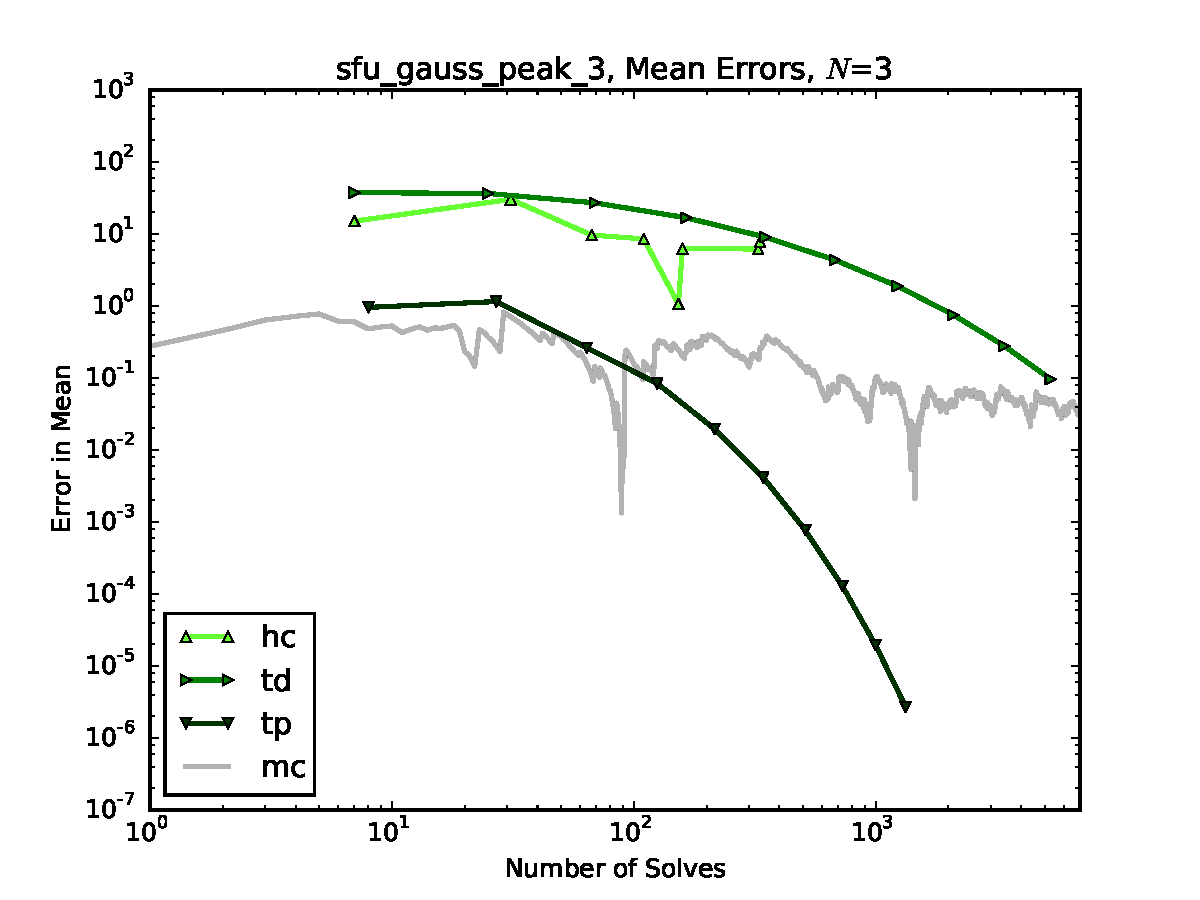
\includegraphics[width=0.7\linewidth]{anlmodels/sfu_gauss_peak_3_mean_errs}
  \caption{Gauss Peak, $N=3$, Mean Convergence}
  \label{fig:hdmr gauss peak mean errors 3}
\end{figure}
\begin{figure}[H]
  \centering
  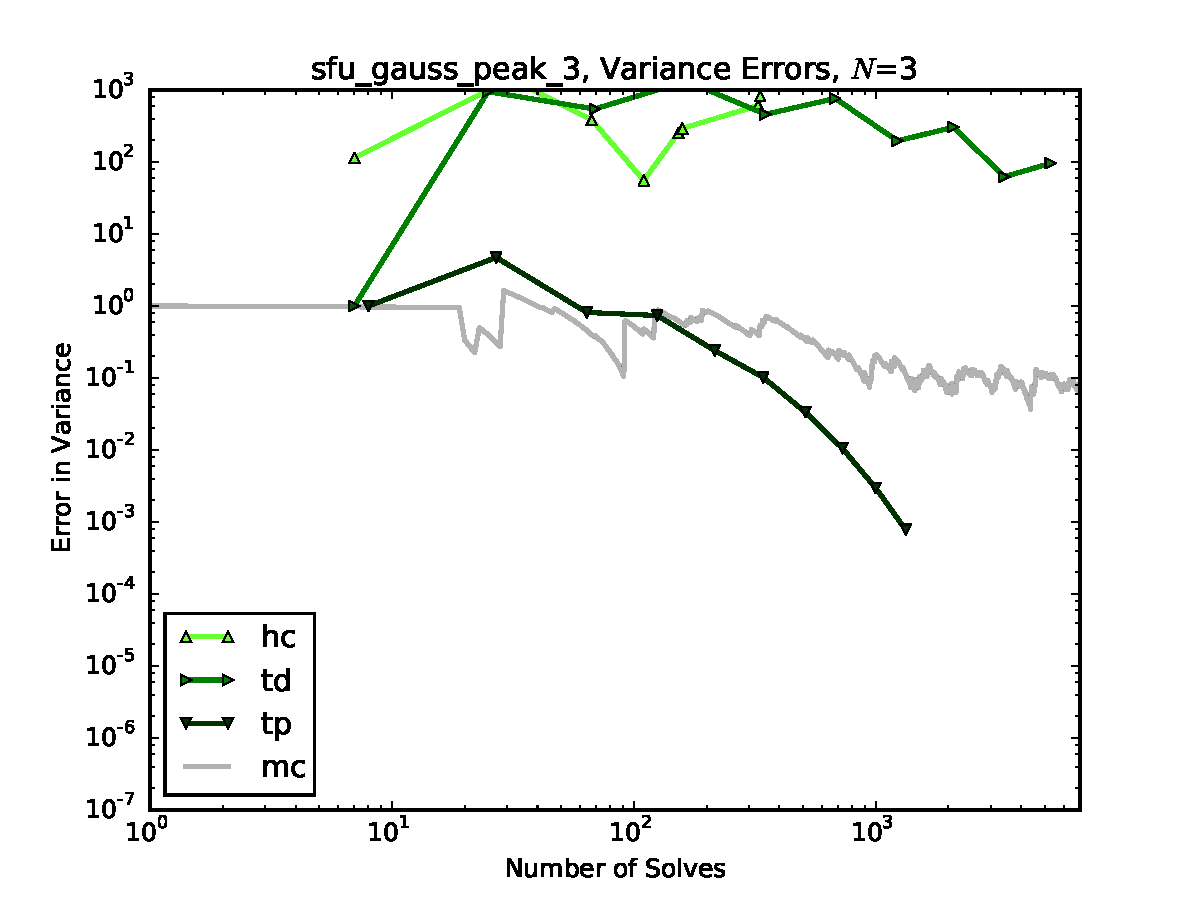
\includegraphics[width=0.7\linewidth]{anlmodels/sfu_gauss_peak_3_variance_errs}
  \caption{Gauss Peak, $N=3$, Std. Dev. Convergence}
  \label{fig:hdmr gauss peak var errors 3}
\end{figure}

\subsection{5 Inputs}
The same trends for the three-input case are observed here for the five-input case, and exacerbated.  This
model requires a great number of high-order, tensor-product polynomials to produce an accurate surrogate, and
neither HDMR nor SCgPC methods are well-equipped to provides them efficiently.
\begin{figure}[H]
  \centering
  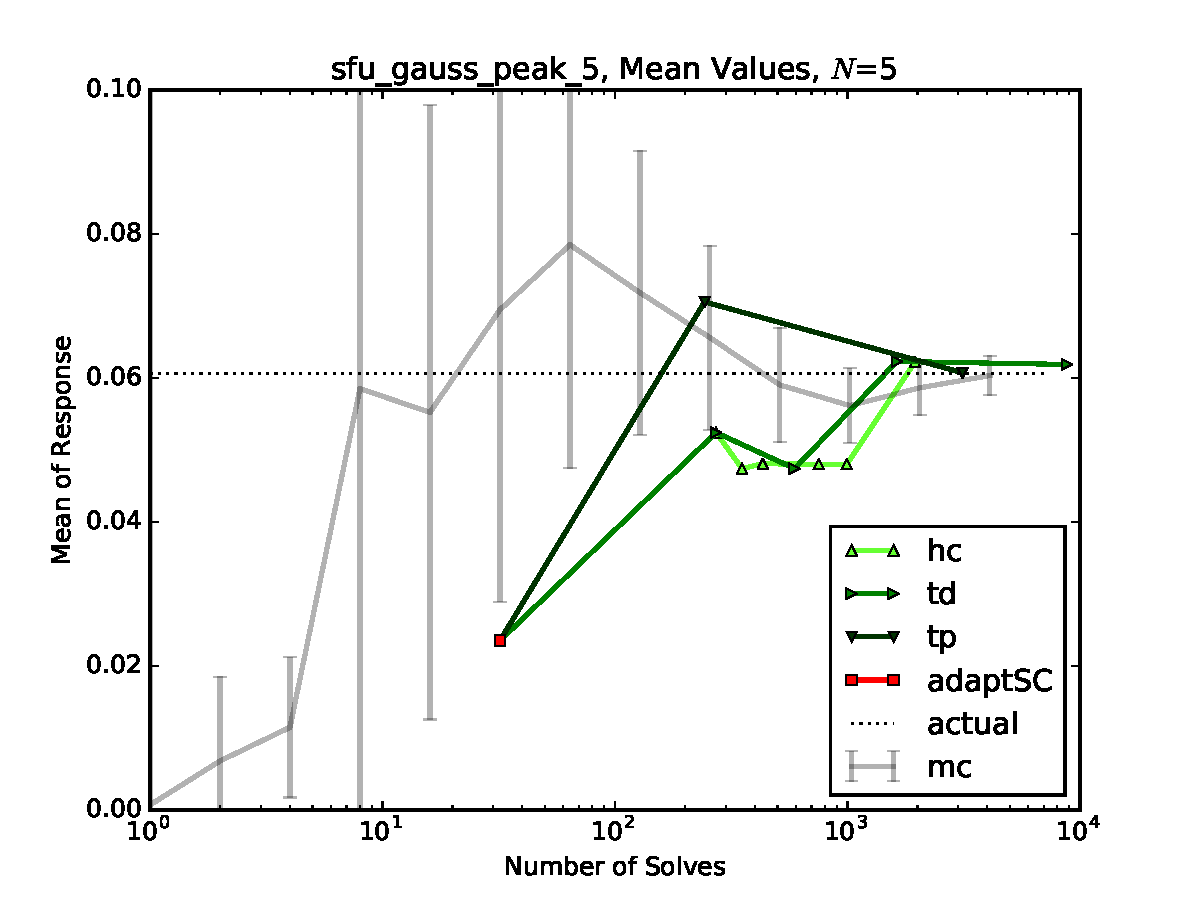
\includegraphics[width=0.7\linewidth]{anlmodels/sfu_gauss_peak_5_mean_vals}
  \caption{Gauss Peak, $N=5$, Mean Values}
  \label{fig:hdmr gauss peak mean values 5}
\end{figure}
\begin{figure}[H]
  \centering
  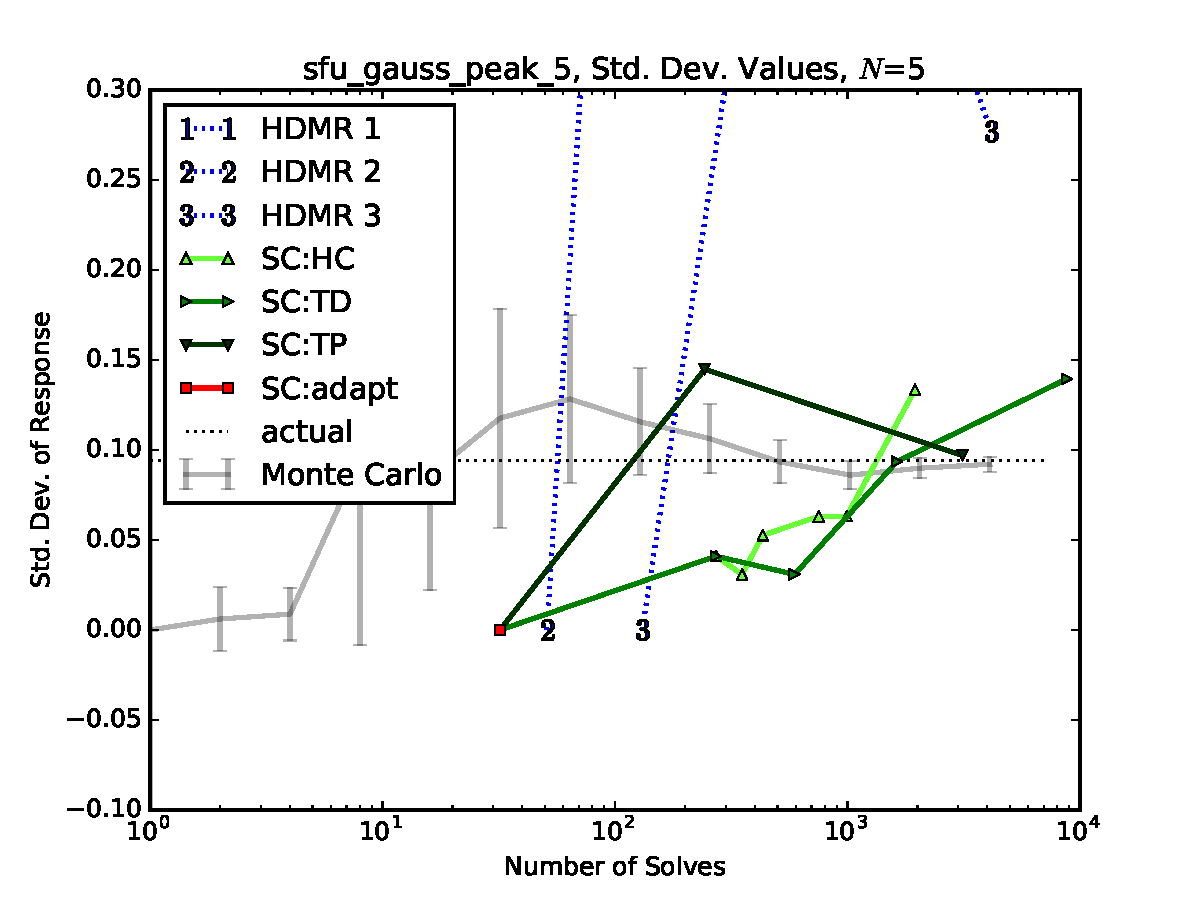
\includegraphics[width=0.7\linewidth]{anlmodels/sfu_gauss_peak_5_var_vals}
  \caption{Gauss Peak, $N=5$, Std. Dev. Values}
  \label{fig:hdmr gauss peak var values 5}
\end{figure}

\begin{figure}[H]
  \centering
  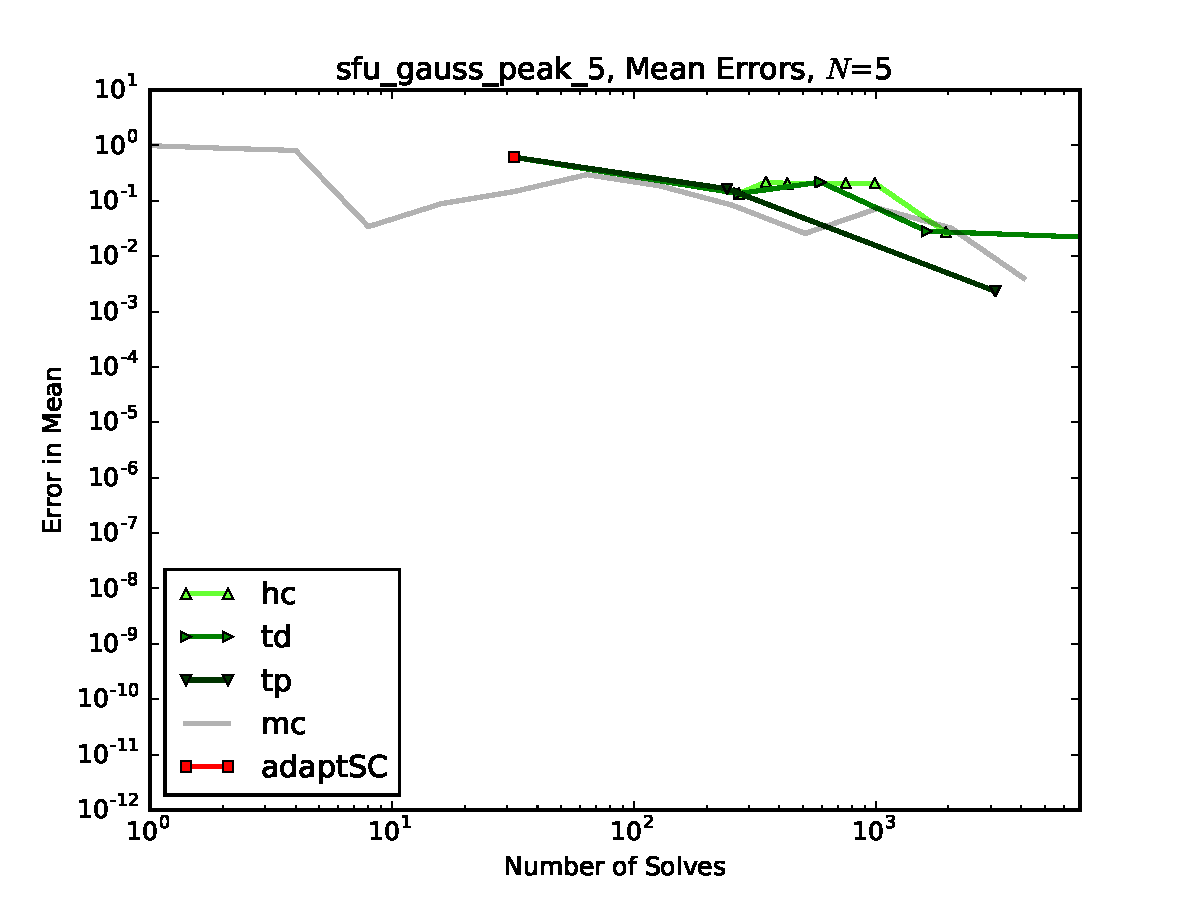
\includegraphics[width=0.7\linewidth]{anlmodels/sfu_gauss_peak_5_mean_errs}
  \caption{Gauss Peak, $N=5$, Mean Convergence}
  \label{fig:hdmr gauss peak mean errors 5}
\end{figure}
\begin{figure}[H]
  \centering
  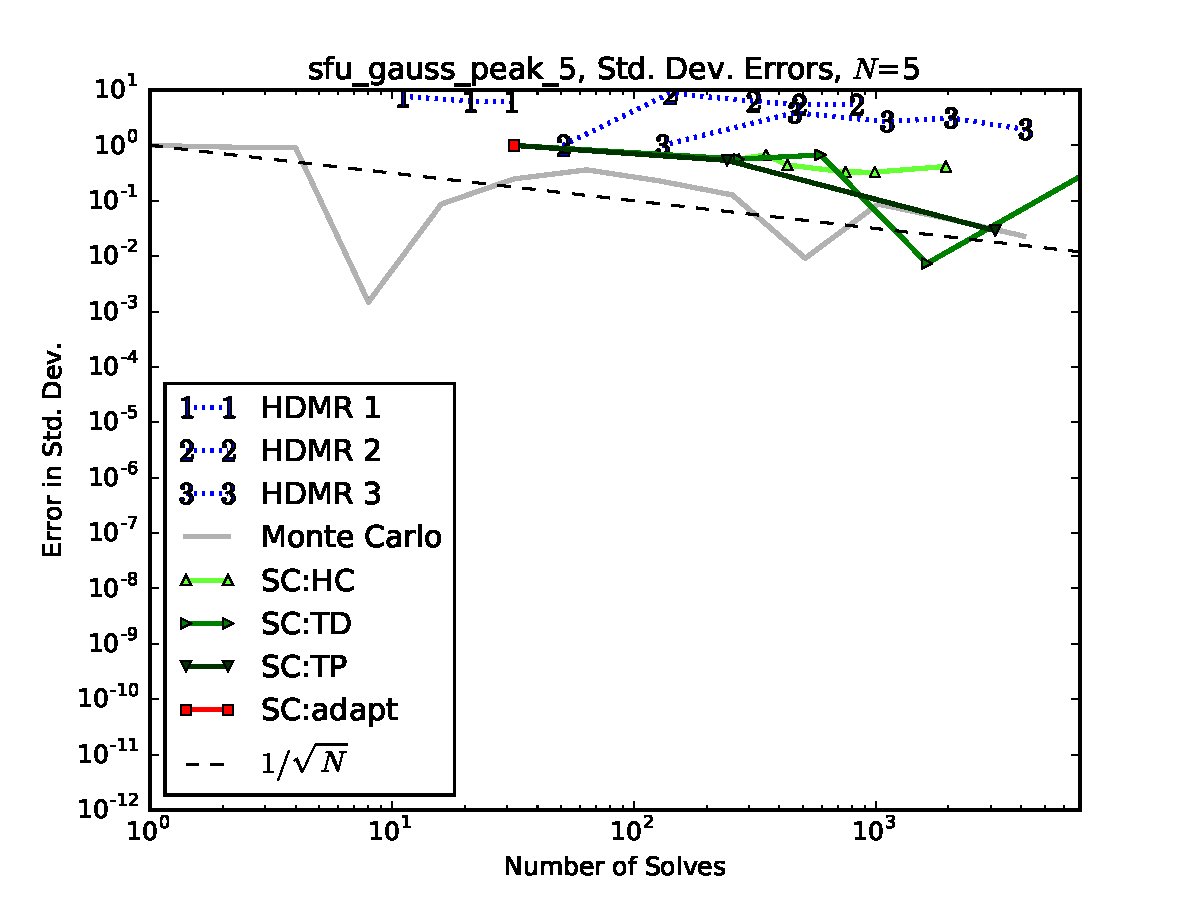
\includegraphics[width=0.7\linewidth]{anlmodels/sfu_gauss_peak_5_variance_errs}
  \caption{Gauss Peak, $N=5$, Std. Dev. Convergence}
  \label{fig:hdmr gauss peak var errors 5}
\end{figure}




\section{Ishigami}
\subsection{3 Inputs}
This model is described in section \ref{mod:ishigami}.
The behavior for the HDMR method on this model are quite interesting.  Because much of this response is
determined by single-order interactions, the static HDMR 1 method converges the mean quite effectively
compared to other methods.  Both HDMR 2 and HDMR 3 also perform well, but HDMR 3 wastes substantial effort as
there are no third-order interactions in this model.  The adaptive HDMR method fails in its search because it
misses the important interaction between $y_3$ and $y_1$, which isn't observed until the fourth-order
polynomial of $y_3$.  Additionally, both $y_1$ and $y_2$ are arguments to sine functions, which when expanded
in polynomials only contain odd powers.  As a result, upon obtaining zero contribution from even-ordered
polynomials, the adaptive algorithm has no metric by which to search for additional contributions.
\begin{figure}[H]
  \centering
  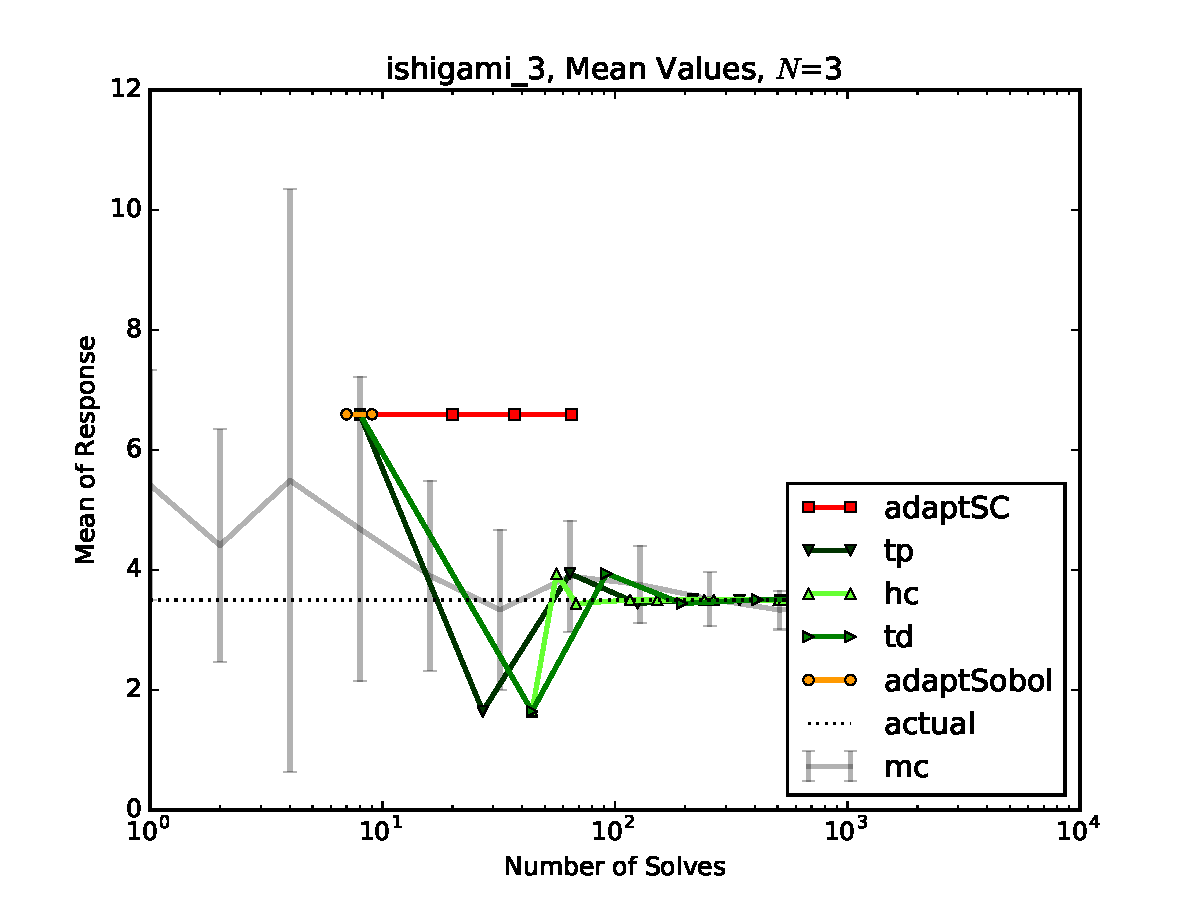
\includegraphics[width=0.7\linewidth]{anlmodels/ishigami_3_mean_vals}
  \caption{Ishigami, $N=3$, Mean Values}
  \label{fig:hdmr ishigami mean values 3}
\end{figure}
\begin{figure}[H]
  \centering
  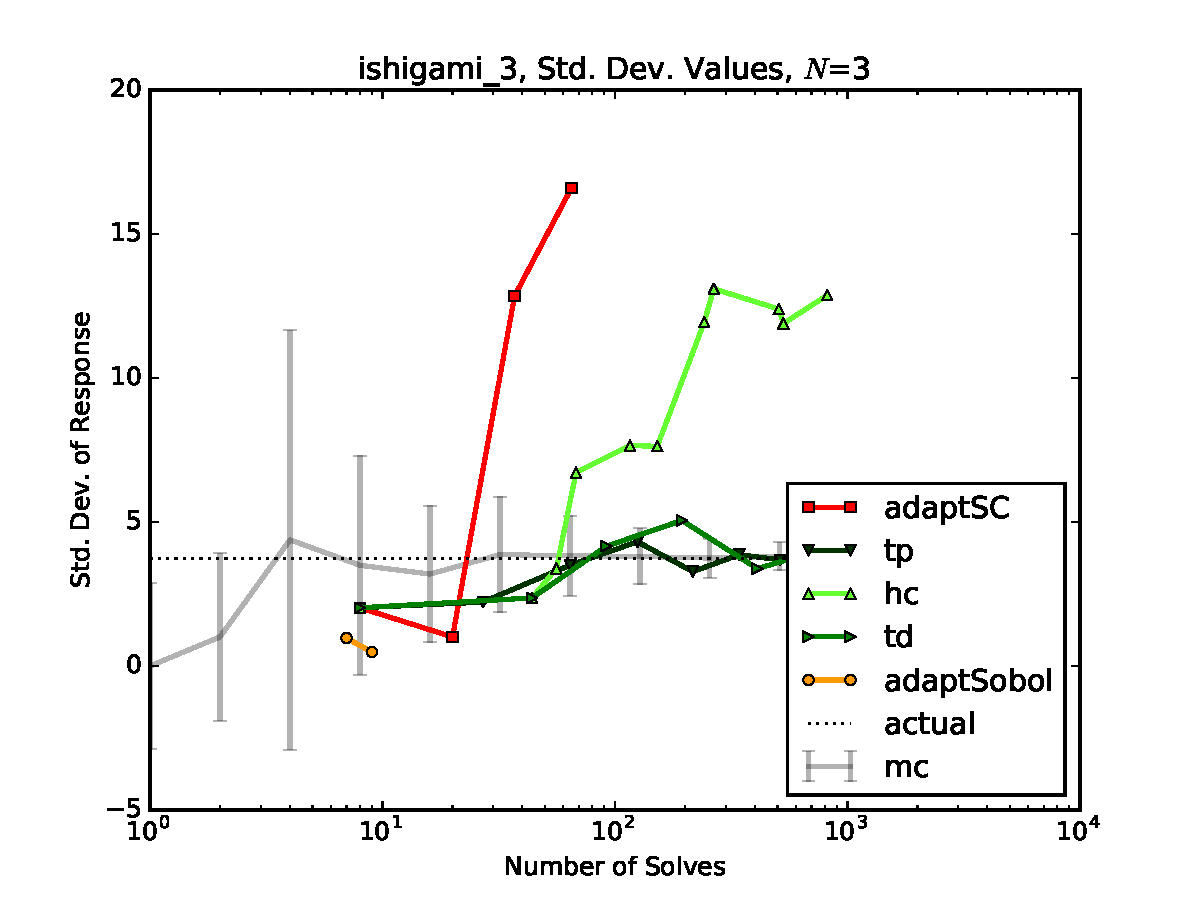
\includegraphics[width=0.7\linewidth]{anlmodels/ishigami_3_var_vals}
  \caption{Ishigami, $N=3$, Std. Dev. Values}
  \label{fig:hdmr ishigami var values 3}
\end{figure}

\begin{figure}[H]
  \centering
  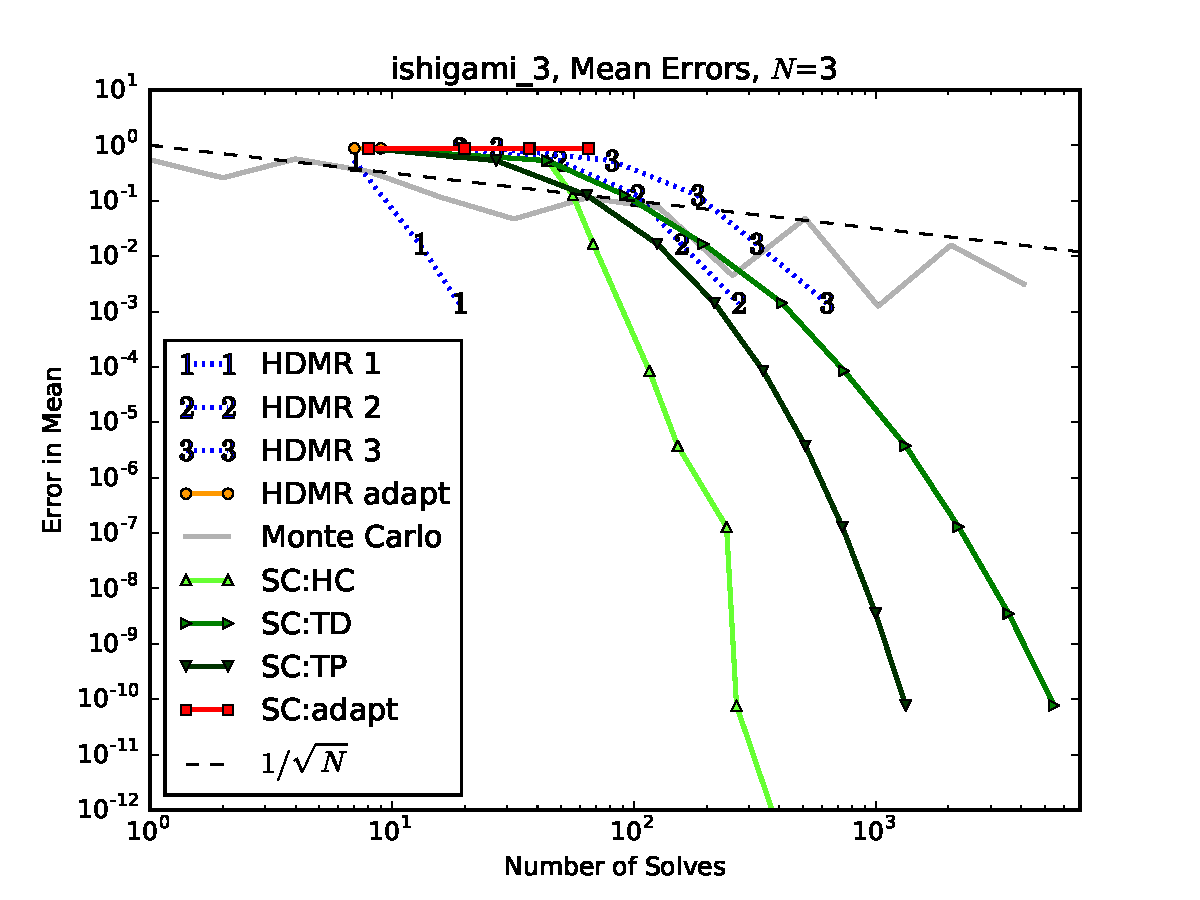
\includegraphics[width=0.7\linewidth]{anlmodels/ishigami_3_mean_errs}
  \caption{Ishigami, $N=3$, Mean Convergence}
  \label{fig:hdmr ishigami mean errors 3}
\end{figure}
\begin{figure}[H]
  \centering
  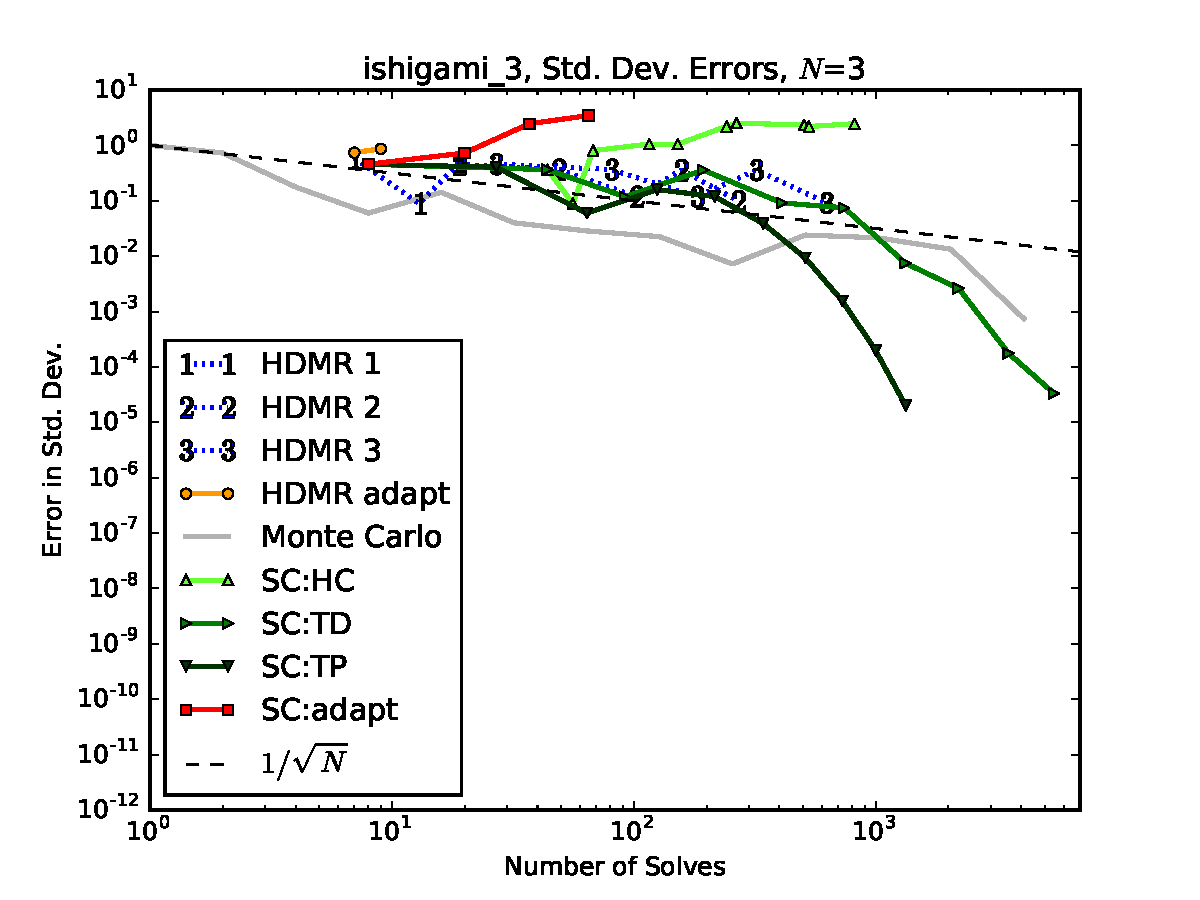
\includegraphics[width=0.7\linewidth]{anlmodels/ishigami_3_variance_errs}
  \caption{Ishigami, $N=3$, Std. Dev. Convergence}
  \label{fig:hdmr ishigami var errors 3}
\end{figure}


\section{Sobol G-Function}
This model is described in section \ref{mod:gfunc}.
Unsurprisingly, this zeroth-order continuous response continues to provide a great challenge to any
polynomial-based method representation.  The adaptive SCgPC and adaptive HDMR methods both fail to converge
more than a single data point, and the static methods all show no clear benefits over traditional Monte Carlo
sampling.
\subsection{3 Inputs}
\begin{figure}[H]
  \centering
  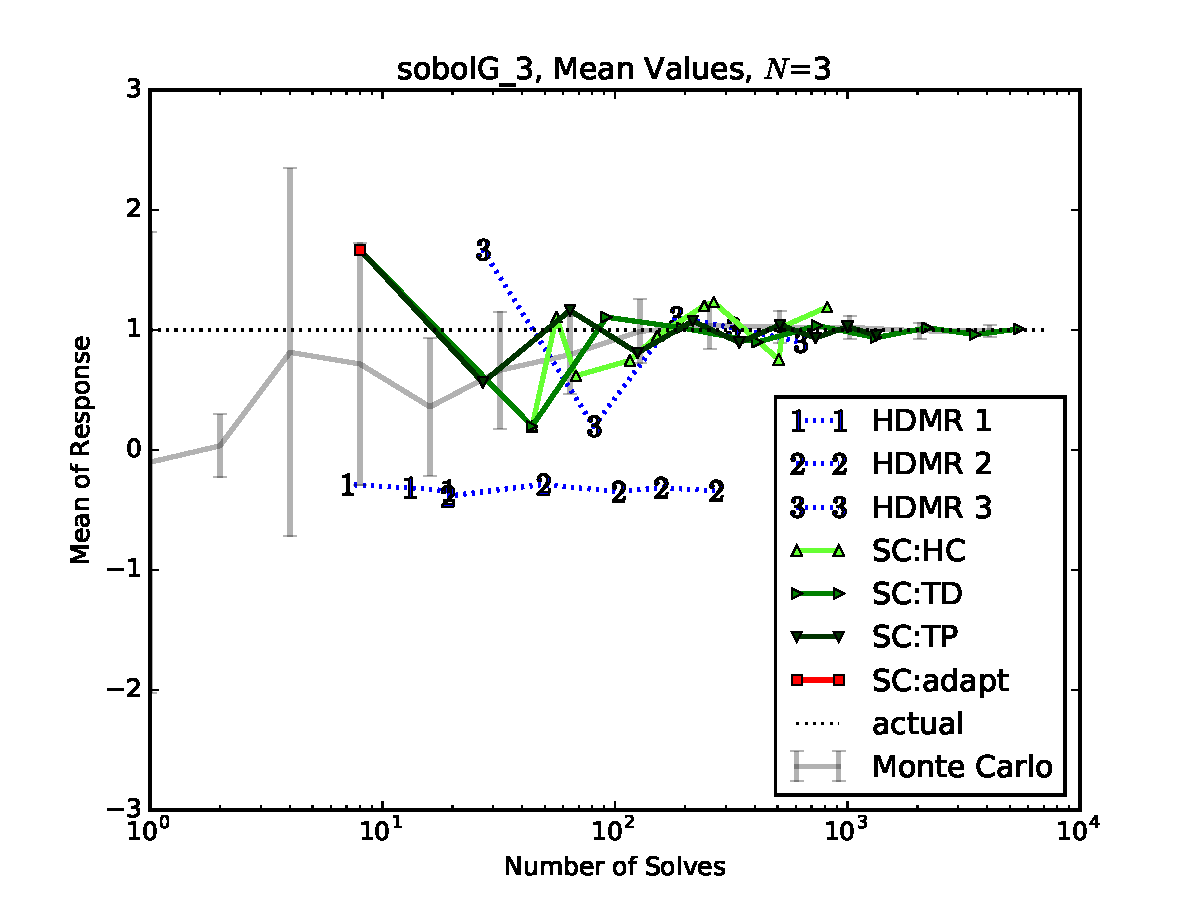
\includegraphics[width=0.7\linewidth]{anlmodels/sobolG_3_mean_vals}
  \caption{Sobol G-Function, $N=3$, Mean Values}
  \label{fig:hdmr sobolG mean values 3}
\end{figure}
\begin{figure}[H]
  \centering
  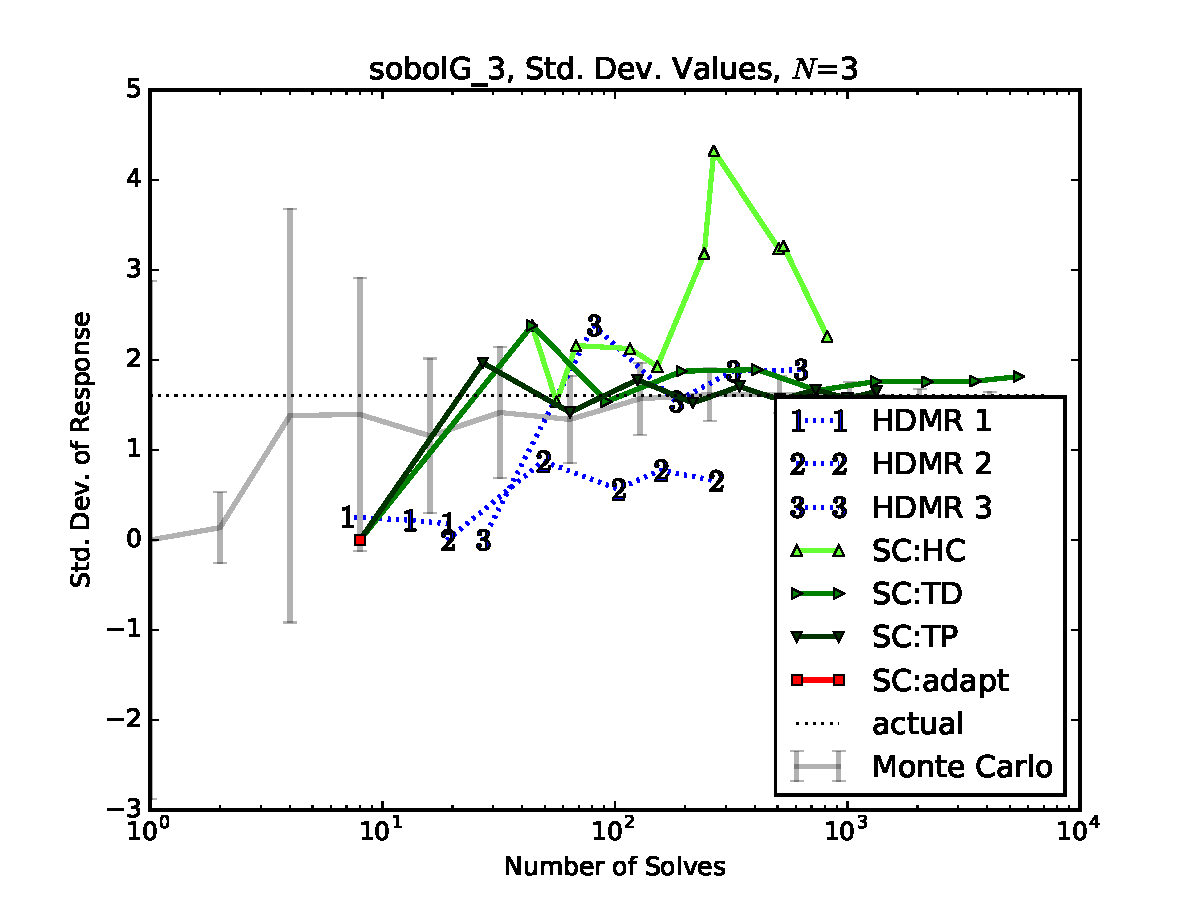
\includegraphics[width=0.7\linewidth]{anlmodels/sobolG_3_var_vals}
  \caption{Sobol G-Function, $N=3$, Std. Dev. Values}
  \label{fig:hdmr sobolG var values 3}
\end{figure}

\begin{figure}[H]
  \centering
  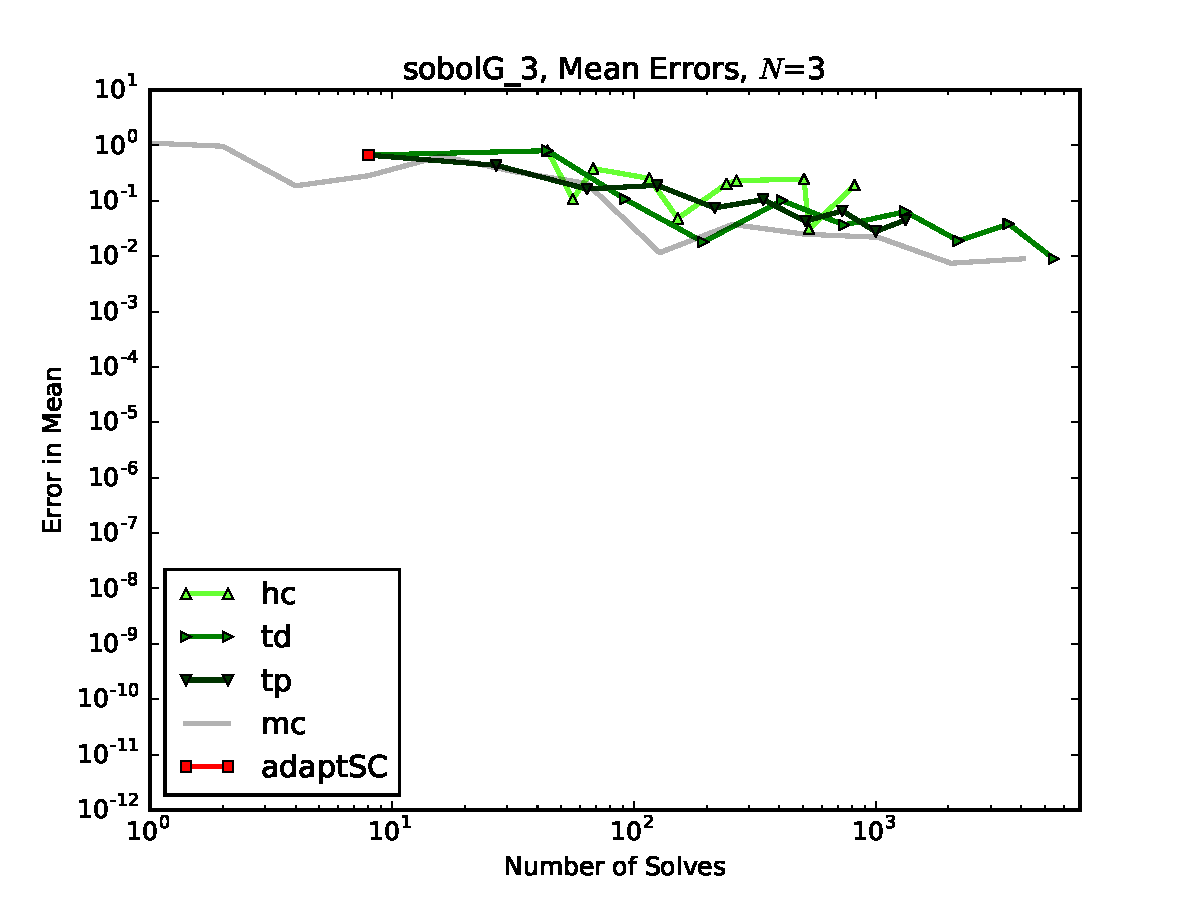
\includegraphics[width=0.7\linewidth]{anlmodels/sobolG_3_mean_errs}
  \caption{Sobol G-Function, $N=3$, Mean Convergence}
  \label{fig:hdmr sobolG mean errors 3}
\end{figure}
\begin{figure}[H]
  \centering
  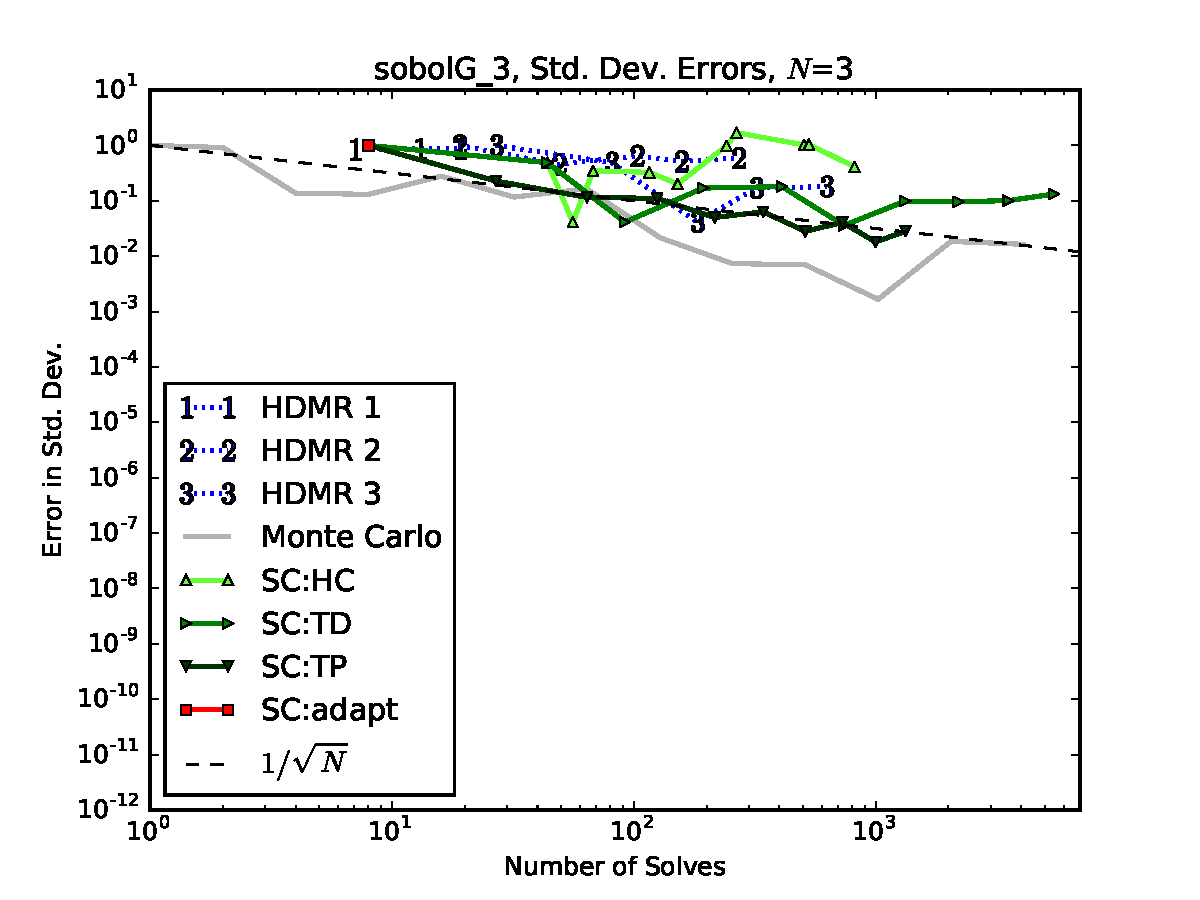
\includegraphics[width=0.7\linewidth]{anlmodels/sobolG_3_variance_errs}
  \caption{Sobol G-Function, $N=3$, Std. Dev. Convergence}
  \label{fig:hdmr sobolG var errors 3}
\end{figure}

\subsection{5 Inputs}
\begin{figure}[H]
  \centering
  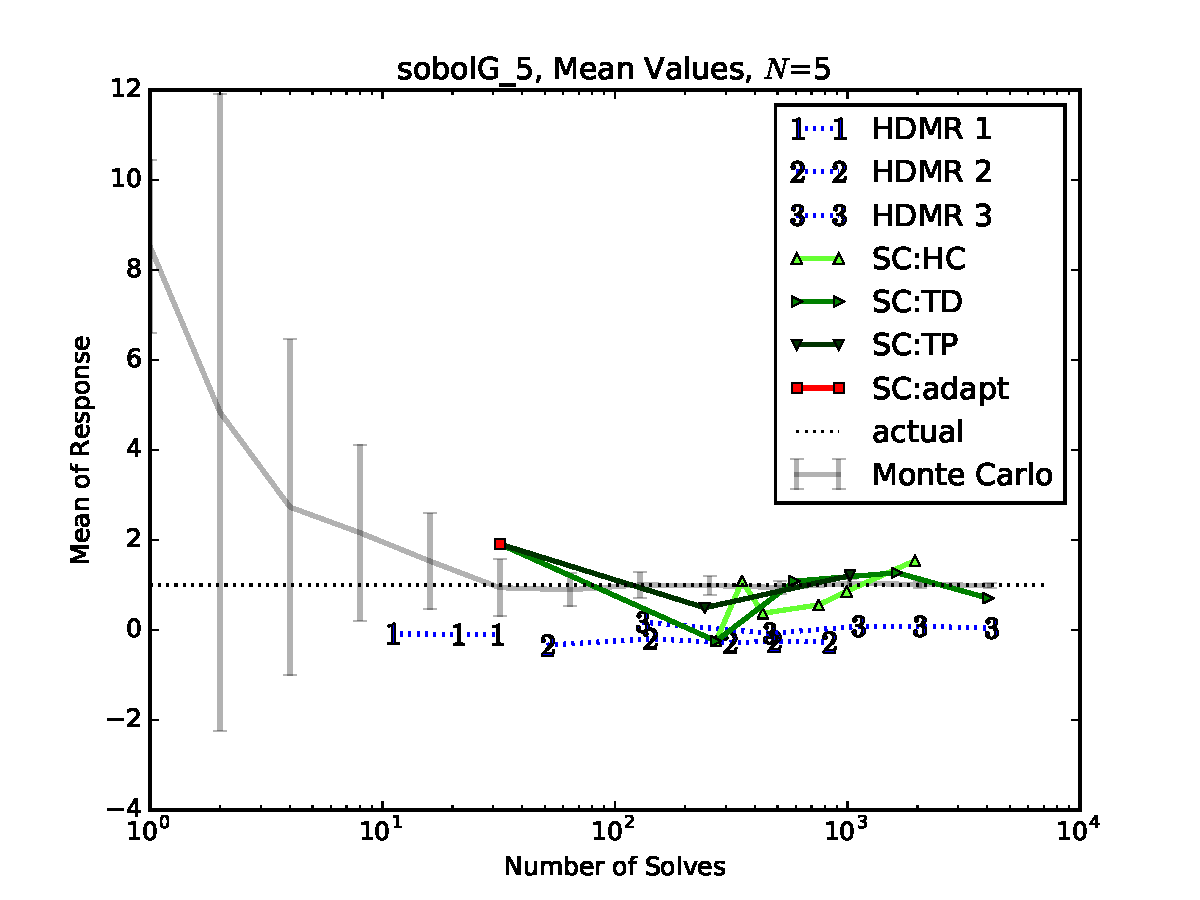
\includegraphics[width=0.7\linewidth]{anlmodels/sobolG_5_mean_vals}
  \caption{Sobol G-Function, $N=5$, Mean Values}
  \label{fig:hdmr sobolG mean values 5}
\end{figure}
\begin{figure}[H]
  \centering
  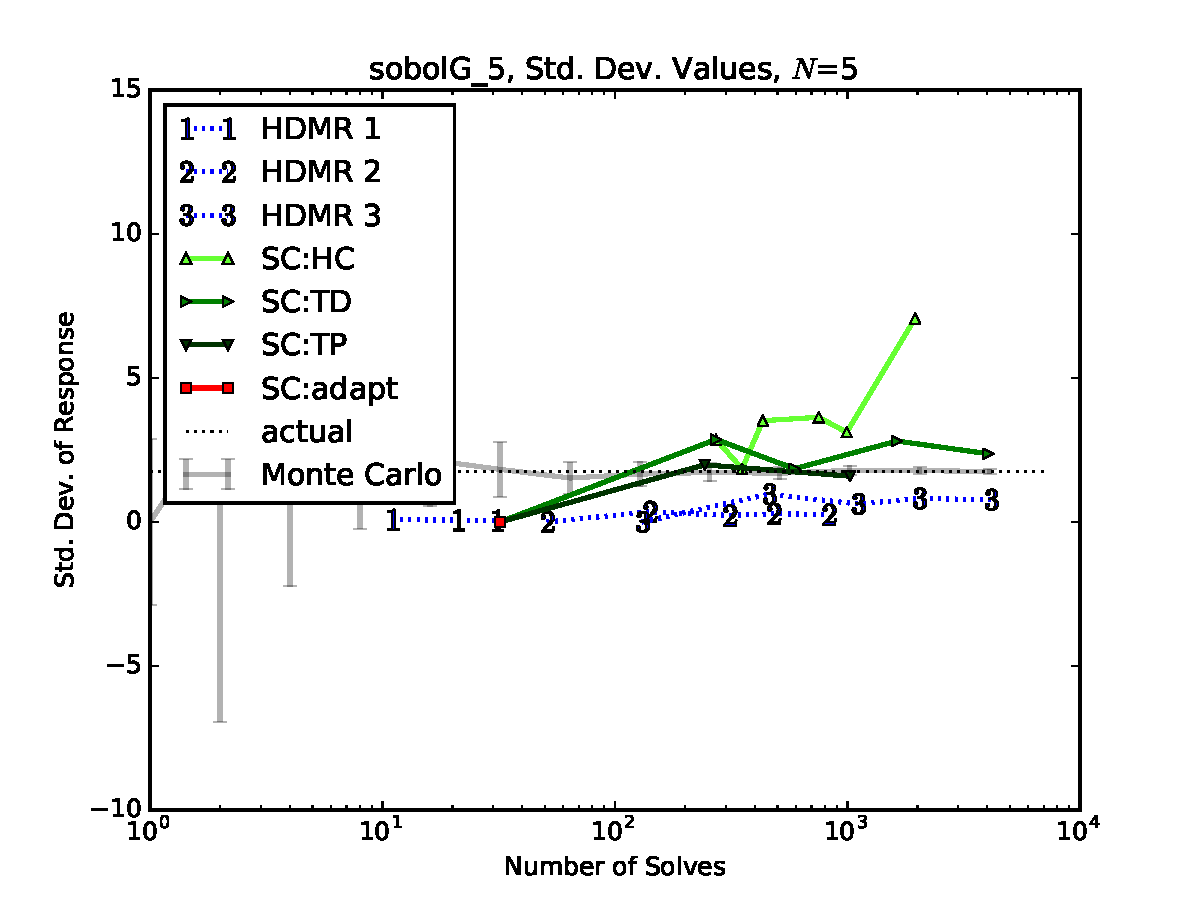
\includegraphics[width=0.7\linewidth]{anlmodels/sobolG_5_var_vals}
  \caption{Sobol G-Function, $N=5$, Std. Dev. Values}
  \label{fig:hdmr sobolG var values 5}
\end{figure}

\begin{figure}[H]
  \centering
  \includegraphics[width=0.7\linewidth]{anlmodels/sobolG_5_mean_errs}
  \caption{Sobol G-Function, $N=5$, Mean Convergence}
  \label{fig:hdmr sobolG mean errors 5}
\end{figure}
\begin{figure}[H]
  \centering
  \includegraphics[width=0.7\linewidth]{anlmodels/sobolG_5_variance_errs}
  \caption{Sobol G-Function, $N=5$, Std. Dev. Convergence}
  \label{fig:hdmr sobolG var errors 5}
\end{figure}


\section{Conclusions}
We have demonstrated the performance of HDMR methods using three different truncation orders as well as
adaptive HDMR subset construction, all based on SCgPC expansions for the HDMR subsets.  We observed good
performance of the adaptive HDMR algorithm when the input space is limit in size and behaves predictably, and
good performance in the static truncated HDMR methods when the interaction terms in the model were limited.
Additionally, we observed that adaptive HDMR and HDMR 1 could obtain UQ solutions with fewer evaluations than
the other SCgPC and HDMR methods, which can be valuable when only very few realizations are practical.

However, in general SCgPC methods outperform HDMR when the input space is regular and isotropic.  This leads
to the conclusion that when computational resources are available, the SCgPC methods may be a better initial choice
than the HDMR methods, while if resources are limited, the adaptive HDMR method can still be a good candidate.
